\documentclass[normal, cyan, en]{elegantnote}
\usepackage{amssymb}
\usepackage{array}
\usepackage{color}
\usepackage{cancel}
\usepackage{minted}
\usepackage{tikz}
\usepackage{algorithmic, algorithm}
\usepackage{xeCJK}
\usepackage{xeCJKfntef}
\usepackage{xcolor}
\usepackage{amsmath, amsfonts, scalerel}
\def\Z{{\mathbb Z}}
\def\R{{\mathbb R}}
\def\C{{\mathbb C}}
\def\Q{{\mathbb Q}}
\def\du{{^{\circ}}}
\definecolor{cool}{RGB}{120,67,131}
\newcommand{\limit}[2]{\lim\limits_{#1 \to #2}}
\newcommand{\Sum}[3]{\sum\limits_{#1 = #2}^{#3}}
\newcommand{\roma}[1]{\uppercase\expandafter{\romannumeral#1}}
\newcommand{\QED}{\square}
\newcommand{\stirling}[2]{\begin{Bmatrix}#1\\#2\end{Bmatrix}}
\newcommand*{\dif}{\mathop{}\!\mathrm{d}}
\usetikzlibrary{arrows, graphs}
% \renewcommand{\textbf}[1]{{\color{red} #1}}
\newcommand{\textbff}[1]{{\color{cool} #1}}
\newcommand\stress[1]{\textbff{\CJKunderdot{#1}}}
\definecolor{custom}{RGB}{128,111,147}
\setcounter{tocdepth}{2}
\DeclareMathOperator*{\btie}{\scalerel*{\bowtie}{\textstyle\sum}}
\title{90 分钟急救机器学习}
\date{\today}

\newminted{sql}{linenos, breaklines, frame = single, mathescape, texcl = true, escapeinside = ||}

\begin{document}

\maketitle
\tableofcontents
\newpage

\section{梯度下降}
梯度下降是一个最优化算法,规范形式为:

\begin{algorithm}[H]
    \renewcommand{\algorithmicrequire}{\textbf{Input:}}
	\renewcommand{\algorithmicensure}{\textbf{Output:}}
    \caption{梯度下降法}
    \begin{algorithmic}[1]
        \REQUIRE $\boldsymbol{\theta}$,$J(\boldsymbol{\theta})$,$\alpha$,其中 $\boldsymbol{\theta}$ 中存储的为随机值
        \ENSURE $\boldsymbol{\theta}$ 为使 $J(\boldsymbol{\theta})$ 取到最小值时的参数
        \WHILE {$\boldsymbol{\theta}$ 不收敛}
            \FOR {$j = 0$ to $n$}
                \STATE $\theta_j := \theta_j - \nabla J(\theta_j)$
            \ENDFOR
        \ENDWHILE
    \end{algorithmic}
\end{algorithm}

\section{线性回归}

\subsection{预测方程}
\begin{equation}
    h_\theta(\boldsymbol{x}) = \sum_{i=0}^n \theta_ix_i
\end{equation}

其中规定 $x_0 = 1$。

若令
\begin{equation}
    \boldsymbol{\theta} = \begin{bmatrix}\theta_0 \\ \theta_1 \\ \vdots \\ \theta_n\end{bmatrix} \in \mathbb R^{n+1},
\boldsymbol{X} = \begin{bmatrix}x_0 \\ x_1 \\ \vdots \\ x_n\end{bmatrix} \in \mathbb R^{n+1}
\end{equation}

则预测方程为
\begin{equation}
    h_\theta(x) = \boldsymbol{\theta}^\mathrm T\boldsymbol{X}
\end{equation}

\subsection{代价函数}
线性回归的代价函数为
\begin{equation}
    J(\theta_j) = \dfrac{1}{2m}\sum_{i=1}^m(h_\theta(\boldsymbol{x}^{(i)}) - y^{(i)})^2
\end{equation}

此时梯度公式为
\begin{equation}
    \nabla J(\boldsymbol{\theta}) = \dfrac{1}{m}\sum_{i=1}^m(h_\theta(\boldsymbol{x}^{(i)}) - y^{(i)})\boldsymbol{x}^{(i)}_j
\end{equation}

\subsection{归一化}
1. 均值归一化为
\begin{equation}
    x_i \leftarrow \dfrac{x_i - \mu_i}{\max - \min}
\end{equation}

2. min-max 归一化为
\begin{equation}
    x_i \leftarrow \dfrac{x_i - \min}{\max - \min}
\end{equation}

\subsection{学习率}
1. 学习率太小时,收敛的速度可能会很慢;

2. 学习率太大时,可能会导致算法不收敛,代价函数 $J(\boldsymbol{\theta})$ 可能不会每次迭代都减小。

\subsection{正规方程法求 $\boldsymbol{\theta}$}

令
\begin{equation}
    X = \begin{bmatrix}1 & x^{(1)}_1 & x^{(1)}_2 & \cdots & x^{(1)}_n \\ 1 & x^{(2)}_1 & x^{(2)}_2 & \cdots & x^{(2)}_n 
        \\ 1 & \vdots & \vdots & \vdots & \vdots \\ 1 & x^{(m)}_1 & x^{(m)}_2 & \cdots & x^{(m)}_n\end{bmatrix} \in \mathbb R^{m \times (n+1)},
    y = \begin{bmatrix}y^{(1)} \\ y^{(2)} \\ \vdots \\ y^{(m)}\end{bmatrix} \in \mathbb R^m
\end{equation}

则
\begin{equation}
    \boldsymbol{\theta} = (X^\mathrm T X)^{-1}X^\mathrm Ty
\end{equation}

考虑到矩阵乘法的复杂度为 $\mathcal O(n^3)$,所以当 $n$ 不是很大时可以考虑使用正规方程法,否则使用梯度下降法。

$X^\mathrm T X$ 不可逆的情况有两种:\par
1. 某些特征之间存在线性关系,导致部分特征是冗余的;

2. 训练集中的样本数目小于特征数目。

\section{逻辑回归}

\subsection{Sigmoid 函数}
Sigmoid 函数为
\begin{equation}
    g(x) = \dfrac{1}{1 + e^{-x}}
\end{equation}

性质:$g(x) \in (0, 1)$,$g(0) = \frac 12$,$\lim\limits_{x \to -\infty}g(x) = 0$,$\lim\limits_{x \to +\infty}g(x) = 1$。

\subsection{预测函数}
\begin{equation}
    h_\theta(\boldsymbol{x}) = g(\boldsymbol{\theta}^\mathrm T\boldsymbol{x} + b)
\end{equation}
    
\subsection{代价函数}
\begin{equation}
    J(\boldsymbol{\theta}) = -\dfrac{1}{m}\sum_{i=1}^m\left[y^{(i)}\log h_\theta(\boldsymbol{x}^{(i)}) + (1 - y^{(i)})\log(1 - h_\theta(\boldsymbol{x}^{(i)}))\right]
\end{equation}

此时梯度公式为
\begin{equation}
    \nabla J(\theta_j) = \dfrac{1}{m}\sum_{i=1}^m(h_\theta(\boldsymbol{x}^{(i)}) - y^{(i)})\boldsymbol{x}^{(i)}_j
\end{equation}

\subsection{多分类问题}
对于多分类问题,可以使用一对多的方法,即对于每个类别 $k$,训练一个逻辑回归分类器。
对于一个输入,只需找到输出最大的那个分类器,并将其对应的类别作为输入的类别。

\section{正则化}
\subsection{概念}
过拟合(overfitting)指的是当有多个特征时,预测函数的代价可能会很低,但对于新的预测数据全都错误的情况,这会导致模型的泛化能力较差。通过进行正则化可以提高模型的\textbf{泛化能力}。

\subsection{LASSO}

以线性回归为例,以平方误差为损失函数,并将岭回归中的 L2 范数替换为 L1 范数,有
\begin{equation}
    \min_{\boldsymbol{w}}\sum\limits_{i=1}^m{(y_i - \boldsymbol{w}^\mathrm T \boldsymbol{x}_i)^2 
    + \lambda \|\boldsymbol{w}\|_1}
\end{equation}
其中正则化参数 $\lambda > 0$,上式称为 LASSO。

LASSO 易获得稀疏解,即它求得的 $\boldsymbol{w}$ 会有更少的非零分量,如下图所示:
\begin{figure}[htbp]
    \centering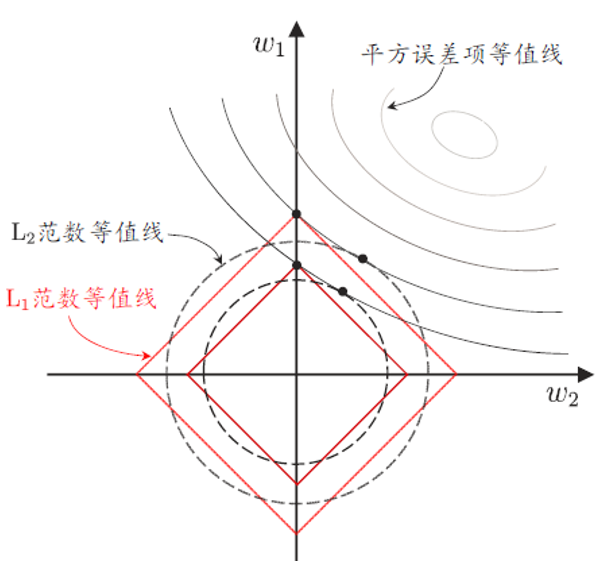
\includegraphics[scale = 0.4]{LASSO.png}
\end{figure}

可以发现,L1 范数的等值线与平方误差项的等值线的交点“常”出现在坐标轴上,即产生一个 $w_1$ 或 $w_2$ 为 0 的稀疏解,
而 L2 范数的等值线与平方误差项的等值线的交点“不太可能”出现在坐标轴上,$w_1$ 和 $w_2$ 都非 0。

\subsection{岭回归}

以线性回归为例,加入 L2 正则项后的代价函数为
\begin{equation}
    J(\boldsymbol{\theta}) = \dfrac{1}{2m}\sum_{i=1}^m(h_\theta(\boldsymbol{x}^{(i)}) - y^{(i)})^2 + \dfrac{\lambda}{2m}\sum_{\textcolor{red}{j=1}}^n\theta_j^2
\end{equation}

其中 $\lambda$ 称为正则化参数,$\lambda\sum\limits_{\textcolor{red}{j=1}}^n\theta_j^2$ 被称为 L2 正则项。

如果正则化参数过大,惩罚的程度过高,我们会得到一个除了 $\theta_0$ 以外,其他的参数都趋于零的结果,
相当于把假设函数的全部项都忽略掉了,这就导致了欠拟合的现象,欠拟合会导致\textbf{高偏差}。

如果正则化参数过小,惩罚的程度过低,相当于没有进行正则化,这就导致了过拟合的现象,过拟合会导致\textbf{高方差}。

\subsection{使用岭回归对线性回归进行正则化}
1. 梯度下降法:加入正则项后的梯度下降式为
\begin{equation}
    \begin{aligned}
        \theta_0 &:= \theta_0 - \alpha \dfrac 1m \sum\limits_{i = 1}^m {\left(h_\theta(x^{(i)}) - y^{(i)}\right)}x_0^{(i)} \\
        \theta_j &:= \theta_j - \alpha \left[\dfrac 1m \sum\limits_{i = 1}^m {\left(h_\theta(x^{(i)}) - y^{(i)}\right)}x_j^{(i)} + \dfrac{\lambda}{m}\theta_j\right]\ (j = 1, 2, 3, \dots, n) \\
        &:=\theta_{j}\left(1-\alpha \dfrac{\lambda}{m}\right)-\alpha \dfrac{1}{m} \sum_{i=1}^{m}\left(h_{\theta}\left(x^{(i)}\right)-y^{(i)}\right) x_{j}^{(i)}
    \end{aligned}
\end{equation}

2. 正规方程法:加入正则项后 $\boldsymbol{\theta}$ 的解为
\begin{equation}
    \boldsymbol\theta = \left(\mathbf{X}^{\mathrm{T}}\mathbf{X} + \lambda \begin{bmatrix}0 & & & & & \\ & 1 & & & & 
        \\ & & 1 & & & \\ & & & 1 & & \\& & & & \ddots & 
        \\ & & & & & 1\end{bmatrix}\right)^{-1}\mathbf{X}^{\mathrm{T}}y
\end{equation}

矩阵为一个主对角线上除了第一行第一列元素为 $0$,其他全为 $1$ 的 $(n + 1) \times (n + 1)$ 的矩阵。

\subsection{使用岭回归对逻辑回归进行正则化}
加入正则项后的梯度下降式为
\begin{equation}
    \begin{aligned}
        \theta_0 &:= \theta_0 - \alpha \dfrac 1m\sum\limits_{i = 1}^m\left(h_\theta\left(x^{(i)}\right) - y^{(i)}\right)x_0^{(i)} \\
        \theta_j &:= \theta_j - \alpha \left[\dfrac 1m\sum\limits_{i = 1}^m\left(h_\theta\left(x^{(i)}\right) 
        - y^{(i)}\right)x_j^{(i)} + \dfrac \lambda m \theta_j\right],\ (j = 1, 2, 3, \dots, n) \\
        &:= \left(1 - \alpha\dfrac\lambda m\right)\theta_j - \alpha \dfrac 1m\sum\limits_{i = 1}^m\left(h_\theta\left(x^{(i)}\right) 
        - y^{(i)}\right)x_j^{(i)}
    \end{aligned}
\end{equation}

\section{Softmax 回归}

Softmax 回归用于多分类问题,如果分类的类别是互斥的,适于选择 softmax 回归分类器。
如果类别之间不是互斥的,而是相互掺杂,则 k 个 logistic 回归分类器更加合适。当 $k = 2$ 时,Softmax 回归退化为逻辑回归。

\subsection{假设函数}
\begin{equation}
    h_\theta\left(x^{(i)}\right) = 
\begin{bmatrix}
p(y^{(i)}=1 \mid x^{(i)};\theta \\
p(y^{(i)}=2 \mid x^{(i)};\theta \\
\vdots \\
p(y^{(i)}=k \mid x^{(i)};\theta)
\end{bmatrix}
= \dfrac{1}{\sum_{j=1}^k e^{\theta_j^\mathrm Tx^{(i)}}}
\begin{bmatrix}
e^{\theta_1^\mathrm Tx^{(i)}} \\
e^{\theta_2^\mathrm Tx^{(i)}} \\
\vdots \\
e^{\theta_k^\mathrm Tx^{(i)}}
\end{bmatrix}
\end{equation}

其中 $\theta_1, \theta_2, \cdots, \theta_k \in \mathbb{R}^{n+1}$。

\subsection{代价函数}
若令 $\boldsymbol{\theta} =
\begin{bmatrix}
\theta_1^\mathrm T \\
\theta_2^\mathrm T \\
\vdots \\
\theta_k^\mathrm T
\end{bmatrix}_{k \times (n + 1)}$,则代价函数为
\begin{equation}
    J(\boldsymbol{\theta}) = -\dfrac 1m \left(\sum_{i=1}^m\sum_{j=1}^k1\left[y^{(i)} = j\right]\log 
    \dfrac{e^{\theta_j^\mathrm Tx^{(i)}}}{\sum_{l=1}^k e^{\theta_l^\mathrm Tx^{(i)}}}\right)
\end{equation}

其中 $1[x]$ 为示性函数,表示 $x$ 为真时为 $1$,否则为 $0$。

\subsection{梯度下降}
在 Softmax 回归中,将 $x$ 归类为类别 $j$ 的概率为
\begin{equation}
    p\left(y^{(i)}=j \mid x^{(i)} ; \theta\right)
    =\frac{e^{\theta_{j}^{\mathrm T} x^{(i)}}}{\sum_{l=1}^{k} e^{\theta_{l}^{\mathrm T} x^{(i)}}}
\end{equation}

则梯度公式为
\begin{equation}
    \nabla_{\theta_{j}} J(\boldsymbol\theta)=-\frac{1}{m} 
    \sum_{j=1}^{m}1\left[x^{(i)}\left(\left[y^{(i)}=j\right]-p\left(y^{(i)}=j \mid x^{(i)} ; \theta\right)\right)\right]
\end{equation}

\subsection{权重衰减}
所谓权重衰减,事实上就是正则化。
\begin{equation}
    J(\boldsymbol{\theta}) = -\dfrac 1m \left(\sum_{i=1}^m\sum_{j=1}^k1\left[y^{(i)} = j\right]\log \dfrac{e^{\theta_j^\mathrm Tx^{(i)}}}{\sum_{l=1}^k 
    e^{\theta_l^\mathrm Tx^{(i)}}}\right) + \textcolor{red}{\dfrac \lambda 2\sum_{i=1}^k\sum_{j=0}^n\theta_{ij}^2}
\end{equation}

此时梯度公式为
\begin{equation}
    \nabla_{\theta_{j}} J(\boldsymbol\theta)=-\frac{1}{m} \sum_{j=1}^{m}
    \left[x^{(i)}\left(1\left[y^{(i)}=j\right]-p\left(y^{(i)}=j \mid x^{(i)} ; \theta\right)\right)\right] 
    + \textcolor{red}{\lambda \theta_j}
\end{equation}

\section{决策树}
\subsection{基本算法流程}
\begin{algorithm}[H]
    \renewcommand{\algorithmicrequire}{\textbf{Input:}}
	\renewcommand{\algorithmicensure}{\textbf{Output:}}
    \caption{决策树学习基本算法 $\text{TreeGenerate(D, A)}$}
    \begin{algorithmic}[1]
        \REQUIRE 训练集 $D = \left\{(x_1, y_1), (x_2, y_2), \dots, (x_m, y_m)\right\}$ \\ \qquad 属性集 $A = \left\{a_1, a_2, \dots, a_d\right\}$
        \ENSURE 以 node 为根结点的一棵决策树
        \STATE 生成结点 node;
        \IF{$D$ 中样本全属于同一类别 $C$}
        \STATE 将 node 标记为 $C$ 类叶结点;
        \STATE \textbf{return}
        \ENDIF
        \IF{$A = \varnothing$ \textbf{OR} $D$ 中样本在 $A$ 上取值相同}
        \STATE 将 node 标记为叶结点,其类别标记为 $D$ 中样本数最多的类;
        \STATE \textbf{return}
        \ENDIF
        \STATE 从 $A$ 中选择最优划分属性 $a_*$;
        \FOR{$a_*$ 中的每一个值 $a_*^v$}
        \STATE 为 node 生成一个分支;
        \STATE 令 $D_v$ 表示 $D$ 中在 $a_*$ 上取值为 $a_*^v$ 的样本子集;
        \IF{$D_v$ 为空}
        \STATE 将分支结点标记为叶结点,其类别标记为 $D$ 中样本最多的类;
        \STATE \textbf{return}
        \ELSE
        \STATE 以 $\text{TreeGenerate}\left(D_v, A \backslash \left\{a_*\right\}\right)$ 为分支结点;
        \ENDIF
        \ENDFOR
    \end{algorithmic}
\end{algorithm}
\subsection{划分选择}
\subsubsection{信息增益}
令信息熵
\begin{equation}
    \operatorname{Ent}(D) = -\sum\limits_{k=1}^{|\mathcal{Y}|}p_k\log _2(p_k)
\end{equation}
假设离散属性 $a$ 有 $V$ 个可能的取值 $\left\{a^1, a^2, \dots, a^V\right\}$,如果使用属性 $a$ 为样本集进行划分,则会产生 $V$ 个分支结点,
其中第 $v$ 个分支结点包含了 $D$ 中所有属性为 $a^v$ 的样本,记为 $D^v$。我们用下式表示属性 $a$ 对样本集 $D$ 进行划分所获得的“信息增益”:
\begin{equation}
    \operatorname{Gain}(D, a) = \operatorname{Ent}(D) - \sum\limits_{v = 1}^V
    {\dfrac{|D^v|}{|D|}\operatorname{Ent}(D^v)}
\end{equation}

选择最优属性时我们可以采用属性 $a_* = \underset{a \in A}{\arg\max}\operatorname{Gain}(D, a)$。

\subsubsection{增益率}
由于信息增益准则对\textbf{可取值数目较多}的属性有所偏好,为了避免这种影响,
由 Quinlan 在 1993 年提出的 C4.5 决策树算法不直接使用信息增益,而是使用“增益率”来选择最优划分属性,定义为:
\begin{equation}
    \operatorname{Gain\_ratio}(D, a) = \dfrac{\operatorname{Gain}(D, a)}{\operatorname{IV}(a)}
\end{equation}
其中,$\operatorname{IV}(a)$ 表示属性 $a$ 的“固有值”。
属性 $a$ 的可能取值数目越多(即 $V$ 越大),则 $\operatorname{IV}(a)$ 的值通常会越大:
\begin{equation}
    \operatorname{IV}(a) = -\sum\limits_{v = 1}^V
    {\dfrac{|D^v|}{|D|}\log _2\dfrac{|D^v|}{|D|}}
\end{equation}

需注意的是,增益率准则对\textbf{可取值数目较少}的属性有所偏好,因此,
C4.5 算法采用了一种启发式的做法:先找出信息增益高于平均水平的属性,再从其中选择增益率最高的。

\subsubsection{基尼指数}
数据集 $D$ 的纯度可用基尼值来度量:
\begin{equation}
    \begin{aligned}
        \operatorname{Gini}(D) &= \sum\limits_{k=1}^{|\mathcal Y|}{\sum\limits_{k' \neq k}p_kp_{k'}} \\
        &=1 - \sum\limits_{k=1}^{|\mathcal Y|} p_k^2
        \end{aligned}
\end{equation}
直观上,$\operatorname{Gini}(D)$ 反映了从数据集 $D$ 中随机抽取两个样本,
其类别标记不一致的概率,所以 $\operatorname{Gini}(D)$ 越小,则数据集 $D$ 的纯度越高。

属性 $a$ 的基尼指数定义为
\begin{equation}
    \operatorname{Gini\_index}(D, a) = \sum\limits_{v = 1}^V
    {\dfrac{|D^v|}{|D|}\operatorname{Gini}(D^v)}
\end{equation}

我们选择划分后基尼指数最小的属性作为最优划分属性,即 $a_* = \underset{a \in A}{\arg\min}\operatorname{Gini\_index}(D, a)$。

\subsection{剪枝}
剪枝分为“预剪枝”和“后剪枝”两种。

“预剪枝”是指在决策树生成过程中,对每个结点在划分前进行估计,如果划分后泛化能力无法提升,则停止划分并将当前结点标记为叶结点;

“后剪枝”则是先从训练集生成一棵完整的决策树,然后自下向上地对非叶结点进行考察,
如果把该结点的子树替换为叶结点能提高泛化能力,则将该子树替换为叶结点。

对比:
\begin{itemize}
    \item 时间开销:
    \begin{itemize}
        \item 预剪枝:训练时间开销降低,测试时间开销降低
        \item 后剪枝:训练时间开销增加,测试时间开销降低
    \end{itemize}
    \item 过/欠拟合风险:
    \begin{itemize}
        \item 预剪枝:过拟合风险降低,欠拟合风险增加
        \item 后剪枝:过拟合风险降低,欠拟合风险基本不变
    \end{itemize}
    \item 泛化性能:后剪枝通常优于预剪枝
\end{itemize}

\subsection{连续值处理}
设给定样本集 $D$ 和连续属性 $a$,$a$ 在 $D$ 上出现了 $n$ 个不同的取值,
从小到大排序后记为 $\left\{a^1, a^2, \dots, a^n\right\}$。

我们可考察包含 $n - 1$ 个元素的候选划分点集合(即将区间的中点作为候选划分点)
\begin{equation}
    T_a = \left\{\dfrac{a^i + a^{i + 1}}{2}, 1 \leq i \leq n - 1\right\}
\end{equation}

对于信息增益,我们可以稍加改造得到属性连续时的公式:
\begin{equation}
    \begin{aligned}
        \operatorname{Gain}(D, a) &= \underset{t \in T_a}{\max} \operatorname{Gain}(D, a, t) \\
        &= \underset{t \in T_a}{\max} \operatorname{Ent}(D) - \sum\limits_{\lambda \in \left\{-, +\right\}}{\dfrac{|D_t^\lambda|}{|D|}\operatorname{Ent}(D_t^\lambda)}
        \end{aligned}
\end{equation}

\subsection{缺失值处理}
缺失值的处理涉及到两个问题:

(1)如何在属性值缺失的情况下进行划分属性选择? 

(2)给定划分属性,若样本在该属性上的值缺失,如何对样本进行划分?

给定训练集 $D$ 和属性 $a$,令 $\tilde{D}$ 表示 $D$ 中在属性 $a$ 上没有缺失值的样本子集。对于问题(1),我们可以仅通过 $\tilde{D}$ 来判断属性的优劣。

假定 $a$ 有 $V$ 个可取值 $\left\{a^1, a^2, \dots, a^V\right\}$,令 $\tilde{D}^v$ 表示 $\tilde{D}$ 
中在属性 $a$ 上取值为 $a^v$ 的样本子集,$\tilde{D}_k$ 表示 $\tilde{D}$ 
中属于第 $k$ 类($k = 1, 2, \dots, |\mathcal Y|$)的样本子集,则显然有
\begin{equation}
    \begin{aligned}
        \tilde{D} &= \bigcup\limits_{k=1}^{|\mathcal Y|} \tilde{D}_k \\
        \tilde{D} &= \bigcup\limits_{v=1}^V \tilde{D}^v
        \end{aligned}
\end{equation}

假定我们为每个样本 $x$ 赋予一个权重 $w_x$,并定义
\begin{equation}
    \begin{aligned}
        \rho &= \dfrac{\sum_{x \in \tilde{D}}w_x}{\sum_{x \in D} w_x} \\
        \tilde{p}_k &= \dfrac{\sum_{x \in \tilde{D}_k} w_x}{\sum_{x \in D} w_x}\quad (1 \leq k \leq |\mathcal Y|) \\
        \tilde{r}_v &= \dfrac{\sum_{x \in \tilde{D}^v} w_x}{\sum_{x \in D} w_x}\quad (1 \leq v \leq V)
        \end{aligned}
\end{equation}

$\rho$ 表示无缺失值样本所占的比例,$\tilde{p}_k$ 表示无缺失值样本中第 $k$ 类所占比例,
$\tilde{r}_v$ 表示无缺失值样本中在属性 $a$ 上取值为 $a^v$ 的样本所占的比例。

基于上述定义,我们可将信息增益的计算式推广为
\begin{equation}
  \begin{aligned}
\operatorname{Gain}(D, a) &= \rho \times \operatorname{Gain}(\tilde{D}, a) \\
&= \rho \times \left(\operatorname{Ent}\left(\tilde{D}\right) - \sum\limits_{v=1}^V{\tilde{r}_v\operatorname{Ent}\left(\tilde{D}^v\right)}\right)
\end{aligned}  
\end{equation}

其中
\begin{equation}
    \operatorname{Ent}(\tilde{D}) = -\sum\limits_{k=1}^{|\mathcal Y|}{\tilde{p}_k \log_2 \tilde{p}_k}
\end{equation}

对问题(2):

\begin{itemize}
    \item 若样本 $x$ 在划分属性 $a$ 上的取值已知,则将 $x$ 划入与其取值对应的子结点,且样本权值在子结点中保持为 $w_x$;
    \item 若样本 $x$ 在划分属性 $a$ 上的取值未知,则将 $x$ 同时划入所有子结点,
    且样本权值在与属性值 $a^v$ 对应的子结点中调整为 $\tilde{r}_v \cdot w_x$。
\end{itemize}

\subsection{从“树”到“规则”,从“单变量”到“多变量”}

可以发现,一颗决策树对应着一个“规则集”,每个从根结点到叶结点的分支路径对应于一条规则。
将决策树转化为一个规则集可以改善可理解性,进一步提升泛化能力。

在每个非叶结点仅考虑一个划分属性时得到的决策树称为“\textbf{单变量决策树}”,产生的是“轴平行”分类面,
当分类边界比较复杂时,单变量决策树必须使用很多段划分才能获得较好的近似,此时决策树会相当复杂,时间开销会很大。
若能够使用斜的划分边界,则模型将大为简化,“多变量决策树”可以做到这一点。
在该模型中,每个非叶结点不再是仅对某个属性,而是\textbf{构造一个线性分类器},如此决策树模型可以大为简化。
更复杂地,我们可以在结点上嵌入神经网络或其他非线性模型,获得更优的决策边界。

\section{数据降维-主成分分析}
\subsection{PCA 算法}
主成分分析(Principal Component Analysis,PCA)是最常用的一种降维方法。

对于正交属性空间中的样本点,如果用一个超平面对所有样本进行恰当地表达,它应当具有下列性质:

\begin{itemize}
    \item \textbf{最近重构性}:样本点到这个超平面的距离都足够近;
    \item \textbf{最大可分性}:样本点到这个超平面上的投影能尽可能分开。
\end{itemize}

\begin{algorithm}[H]
    \renewcommand{\algorithmicrequire}{\textbf{Input:}}
	\renewcommand{\algorithmicensure}{\textbf{Output:}}
    \caption{PCA 算法}
    \begin{algorithmic}[1]
        \REQUIRE 样本集 $D = \left\{\boldsymbol{x}_1, \boldsymbol{x}_2, \cdots, \boldsymbol{x}_m\right\}$, 低维空间维数 $d'$
        \ENSURE 投影矩阵 $W = \left\{\boldsymbol{w}_1, \boldsymbol{w}_2, \cdots, \boldsymbol{w}_{d'}\right\}$
        \STATE 对所有样本进行中心化:$\boldsymbol{x}_i \leftarrow \boldsymbol{x}_i - \frac 1m \sum_{i=1}^m \boldsymbol{x}_i$
        \STATE 计算样本的协方差矩阵 $\mathbf{XX}^\mathrm T$
        \STATE 对协方差矩阵 $\mathbf{XX}^\mathrm T$ 做特征值分解
        \STATE 选取前 $d'$ 个最大的特征值对应的特征向量作为投影矩阵 $W$
    \end{algorithmic}
\end{algorithm}

\subsection{特征值分解}
特征值分解:

\begin{itemize}
    \item 先求 $A$ 的特征多项式 $f(\lambda) = |A - \lambda E| = |A - \Lambda|$,
    其中 $\Lambda$ 是一个主对角线上全为 $\lambda$ 的方阵;
    \item 求特征方程 $|A - \lambda E| = 0$ 的全部解,他们就是 $A$ 的全部特征值;
    \item  对于一个特征值 $\lambda_i$,求出相应的特征方程组 $(A - \Lambda_i)X = 0$ 的一组特解
     $\xi_1, \xi_2, \cdots, \xi_t$,则这组解对应的向量即为一个特征向量。
\end{itemize}

降维后低维空间的维数 $d'$ 通常是由用户事先指定,
或通过在 $d'$ 值不同的低维空间中对 k 近邻分类器(或其他开销较小的学习器)进行交叉验证来选取较好的 $d'$ 值。
对 PCA,还可以还可从重构的角度设置一个重构阈值,例如 $t = 95\%$,然后选取使下式成立的最小 $d'$ 值:
\begin{equation}
   \dfrac{\sum_{i=1}^{d'} \lambda_i}{\sum_{i=1}^d{\lambda_i}} \geq t 
\end{equation}


PCA 仅需保留 $\mathbf W$ 与样本的均值向量,即可通过简单的向量减法和矩阵-向量乘法将新样本投影至低维空间中。

降维虽然会导致信息的损失,但一方面舍弃这些信息后能\textbf{使得样本的采样密度增大},
另一方面,当数据受到噪声影响时,最小的特征值所对应的特征向量往往与噪声有关,\textbf{舍弃可以起到去噪效果}。

\section{聚类分析}

\subsection{聚类性能度量}
首先是下面会用到的几个量:
\begin{equation}
    \begin{aligned}
        \mu_i &= \dfrac 1{|C|}\sum\limits_{1 \leq i \leq |C|} \boldsymbol{x}_i \\
        \operatorname{avg}(C) &= \dfrac{2}{|C|(|C|-1)} \sum\limits_{1 \leq i < j \leq |C|} \operatorname{dist}(\boldsymbol{x}_i, \boldsymbol{x}_j) \\
        \operatorname{diam}(C) &= \max_{1 \leq i < j \leq |C|} \operatorname{dist}(\boldsymbol{x}_i, \boldsymbol{x}_j) \\
        d_{\min}(C_i, C_j) &= \min_{\boldsymbol{x}_i \in C_i, \boldsymbol{x}_j \in C_j} \operatorname{dist}(\boldsymbol{x}_i, \boldsymbol{x}_j) \\
        d_{\text{cen}}(C_i, C_j) &= \operatorname{dist}(\mu_i, \mu_j)
        \end{aligned}
\end{equation}

其中,$\operatorname{avg}(C)$ 表示簇 $C$ 内样本间的平均距离,$\operatorname{diam}(C)$ 表示簇 $C$ 内样本间的最远距离,
$d_{\min}(C_i, C_j)$ 表示簇 $C_i$ 和 $C_j$ 最近样本间的距离,$d_{\text{cen}}(C_i, C_j)$ 表示簇 $C_i$ 和 $C_j$ 中心点间的距离,
$\mu_i$ 表示簇 $C$ 的中心点(质心)。

\begin{itemize}
    \item DB 指数:
    \begin{equation}
        \operatorname{DBI} = \dfrac 1k \sum\limits_{i=1}^k{\max_{j \neq i}\left(\dfrac{\operatorname{avg}(C_i)
         + \operatorname{avg}(C_j)}{d_{\text{cen}}(\mu_i, \mu_j)}\right)}
    \end{equation}\par
    DB 指数越小,聚类效果越好。
    \item Dunn 指数:
    \begin{equation}
        \operatorname{DI} = \min_{1 \leq i \leq k}\left\{\min_{j \neq i}\left(\dfrac{d_{\min}(C_i, C_j)}
        {\max\limits_{1 \leq l \leq k}\operatorname{diam}(C_l)}\right)\right\} 
        = \dfrac{\min_{1 \leq k < k' \leq m}d_{\min}(C_k, C_{k'})}{\max_{1 \leq l' \leq m}\operatorname{diam}(C_{l'})}
    \end{equation}\par
    Dunn 指数越大,聚类效果越好。
\end{itemize}

在衡量两个样本$\boldsymbol{x}_i = \left(x_{i1};x_{i2};\dots;x_{in}\right)$ 
和 $\boldsymbol{x}_j = \left(x_{j1};x_{j2};\dots;x_{jn}\right)$ 的距离时,常用的是“闵可夫斯基距离”:
\begin{equation}
    \operatorname{dist}_{\text{mk}}(\boldsymbol{x}_i, \boldsymbol{x}_j)
     = \left(\sum\limits_{u = 1}^n{|x_{iu} - x_{ju}|^p}\right)^{\frac 1p}
\end{equation}

上式即为 $\boldsymbol{x}_i - \boldsymbol{x}_j$ 的 $\boldsymbol{L}_p$ 范数 $\|\boldsymbol{x}_i - \boldsymbol{x}_j\|_p$。
当 $p = 1$ 时,称为“曼哈顿距离”;当 $p = 2$ 时,称为“欧式距离”。

\subsection{原型聚类 - Kmeans 算法}
此类算法假设聚类结构能通过一组原型刻画,在现实聚类任务中极为常用。
通常情况下,算法先对原型进行初始化,再对原型进行迭代更新求解。

Kmeans 算法针对聚类所得的簇划分 $\mathcal{C} = \left\{C_1, C_2, \dots, C_k\right\}$ 最小化均方误差
\begin{equation}
    E = \sum\limits_{i=1}^k{\sum\limits_{\boldsymbol{x} \in C_i} ||\boldsymbol{x} - \mu_i||_2^2}
\end{equation}

其中 $\mu_i = \frac 1{|C_i|}\sum_{\boldsymbol{x} \in C_i} \boldsymbol{x}$ 是簇 $C_i$ 的均值向量,即“原型”。
$E$ 值在一定程度上刻画了簇内样本围绕簇均值向量的紧密程度,$E$ 值越小,则簇内样本相似度越高。

\begin{algorithm}[H]
    \renewcommand{\algorithmicrequire}{\textbf{Input:}}
	\renewcommand{\algorithmicensure}{\textbf{Output:}}
    \caption{$k$-Means 算法}
    \begin{algorithmic}[1]
        \REQUIRE 样本集 $D = \left\{\boldsymbol{x}_1, \boldsymbol{x}_2, \cdots, \boldsymbol{x}_m\right\}$,聚类簇数 $k$
        \ENSURE 簇划分 $\mathcal C = \left\{C_1, C_2, \dots, C_k\right\}$
        \STATE 从 $D$ 中随机选择 $k$ 个样本作为初始均值向量 $\left\{\boldsymbol{\mu}_1, \boldsymbol{\mu}_2, \cdots, \boldsymbol{\mu}_k\right\}$
        \WHILE{当前均值向量被更新或第一次进入循环}
        \STATE 令 $C_i = \varnothing(1 \leq i \leq k)$
        \FOR{$j = 1, 2, \cdots, m$}
            \STATE 计算样本 $\boldsymbol{x}_j$ 与各均值向量 $\boldsymbol{\mu}_i(1 \leq i \leq k)$ 的距离:
            $d_{ji} = \|\boldsymbol{x}_j - \boldsymbol{\mu}_i\|_2$
            \STATE 根据距离最近的均值向量确定 $\boldsymbol{x}_j$ 的簇标记:
            $\lambda_j = \arg\min_{i \in \left\{1, 2, \cdots, k\right\}}d_{ji}$
            \STATE 将样本 $\boldsymbol{x}_j$ 划入对应的簇: 
            $C_{\lambda_j} = C_{\lambda_j} \bigcup \left\{\boldsymbol{x}_j\right\}$
        \ENDFOR
        \FOR{$i = 1, 2, \cdots, k$}
            \STATE 计算新的均值向量 
            $\boldsymbol{\mu}_i' = \frac 1{|C_i|}\sum_{\boldsymbol{x} \in C_i} \boldsymbol{x}$
            \IF{$\boldsymbol{\mu}_i' \neq \boldsymbol{\mu}_i$}
                \STATE 将当前均值向量 $\boldsymbol{\mu}_i$ 更新为 $\boldsymbol{\mu}_i'$
            \ELSE
                \STATE 保持当前均值向量不变
            \ENDIF
        \ENDFOR
        \ENDWHILE
    \end{algorithmic}
\end{algorithm}

\subsection{密度聚类 - DBSCAN 算法}
此类算法假设聚类结构能通过样本分布的紧密程度来确定。
通常情况下,密度聚类算法从样本密度的角度来考察样本之间的可连接性,并基于可连接样本不断扩展聚类簇来获得最终的聚类结果。

DBSCAN 算法是一种著名的密度聚类算法,它基于一组“邻域”参数 $(\epsilon, MinPts)$ 来刻画样本分布的紧密程度。
给定数据集 $D = \left\{\boldsymbol{x}_1, \boldsymbol{x}_2, \dots, \boldsymbol{x}_m\right\}$,定义下面几个概念:
\begin{itemize}
    \item $\epsilon$-邻域:对 $\boldsymbol{x}_j \in D$,其 $\epsilon$-邻域包含样本集 $D$ 中与 $\boldsymbol{x}_j$ 的距离不大于 $\epsilon$ 的样本,
    即 $N_{\epsilon}\left(\boldsymbol{x}_{j}\right)=\left\{\boldsymbol{x}_{i} \in D \mid \operatorname{dist}\left(\boldsymbol{x}_{i}, \boldsymbol{x}_{j}\right) \leqslant \epsilon\right\}$;
    \item 核心对象:若 $\boldsymbol{x}_j$ 的 $\epsilon$-邻域至少包含 $MinPts$ 个样本,
    即 $\left|N_\epsilon(\boldsymbol{x}_j)\right| \geq MinPts$,则 $\boldsymbol{x}_j$ 是一个核心对象;
    \item 密度直达:若 $\boldsymbol{x}_j$ 在 $\boldsymbol{x}_i$ 的 $\epsilon$-邻域中,
    且 $\boldsymbol{x}_i$ 是核心对象,则称 $\boldsymbol{x}_j$ 由 $\boldsymbol{x}_i$ 密度直达;
    \item 密度可达:对 $\boldsymbol{x}_i$ 与 $\boldsymbol{x}_j$,若存在样本序列 $\boldsymbol{p}_1, \boldsymbol{p}_2, \dots, \boldsymbol{p}_n$,其中 $\boldsymbol{p}_1 = \boldsymbol{x}_i$,$\boldsymbol{p}_n = \boldsymbol{x}_j$ 
    且 $\boldsymbol{p}_{i+1}$ 由 $\boldsymbol{p}_i$ 密度直达,则称 $\boldsymbol{x}_j$ 由 $\boldsymbol{x}_i$ 密度可达;
    \item 密度相连:对 $\boldsymbol{x}_i$ 和 $\boldsymbol{x}_j$,若存在 $\boldsymbol{x}_k$ 使得 $\boldsymbol{x}_i$ 
    与 $\boldsymbol{x}_j$ 均由 $\boldsymbol{x}_k$ 密度可达,则称 $\boldsymbol{x}_i$ 与 $\boldsymbol{x}_j$ 密度相连。
\end{itemize}

\begin{figure}[htbp]
    \centering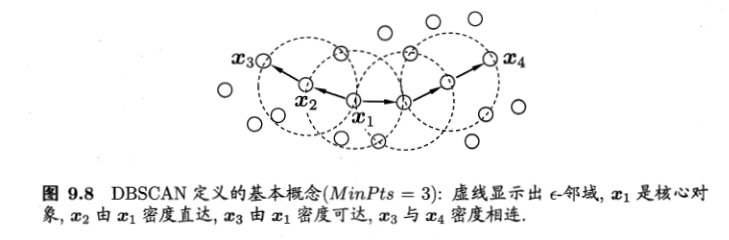
\includegraphics[scale = 0.5]{DBSCAN.png}
\end{figure}

DBSCAN 将“簇”定义为:由密度可达关系导出的最大的密度相连样本集合。

形式化地,给定邻域参数 $(\epsilon, MinPts)$,簇 $C \subseteq D$ 是满足以下性质的非空样本子集:
\begin{itemize}
    \item 连接性:$\boldsymbol{x}_i \in C$,
    $\boldsymbol{x}_j \in C \Longrightarrow$ $\boldsymbol{x}_i$ 和 $\boldsymbol{x}_j$ 密度相连
    \item 最大性:$\boldsymbol{x}_i \in C$,$\boldsymbol{x}_j$ 
    由 $\boldsymbol{x}_i$ 密度可达 $\Longrightarrow$ $\boldsymbol{x}_j \in C$

\end{itemize}

实际上,若 $\boldsymbol{x}$ 为核心对象,则 $\boldsymbol{x}$ 密度可达的所有样本的集合记为 
\begin{equation}
    X = \left\{\boldsymbol{x}' \in D \mid \boldsymbol{x}' \text{由}\boldsymbol{x}\text{密度可达}\right\}
\end{equation}
则 $X$ 即为满足连接性和最大性的簇。

\begin{algorithm}[H]
    \renewcommand{\algorithmicrequire}{\textbf{Input:}}
	\renewcommand{\algorithmicensure}{\textbf{Output:}}
    \caption{DBSCAN 算法}
    \begin{algorithmic}[1]
        \REQUIRE 样本集 $D = \left\{\boldsymbol{x}_1, \boldsymbol{x}_2, \cdots, \boldsymbol{x}_m\right\}$,邻域参数 $(\epsilon, MinPts)$
        \ENSURE 簇划分 $C = \left\{C_1, C_2, \cdots, C_k\right\}$
        \STATE 初始化核心对象集合:$\Omega = \varnothing$
        \FOR{$j = 1, 2, \cdots, m$}
            \STATE 确定 $\boldsymbol{x}_j$ 的 $\epsilon$-邻域 $N_\epsilon(\boldsymbol{x}_j)$
            \IF{$|N_\epsilon(\boldsymbol{x}_j)| \geq MinPts$}
                \STATE 将 $\boldsymbol{x}_j$ 加入核心对象集合:$\Omega = \Omega \bigcup \left\{\boldsymbol{x}_j\right\}$
            \ENDIF
        \ENDFOR
        \STATE 初始化聚类簇数:$k=0$
        \STATE 初始化未访问样本集合:$\Gamma = D$
        \WHILE{$\Omega \neq \varnothing$}
            \STATE 记录当前未访问样本集合:$\Gamma_{\text{old}} = \Gamma$
            \STATE 随机选取一个核心对象 $\boldsymbol{o} \in \Omega$,初始化队列 $Q = <\boldsymbol{o}>$
            \STATE $\Gamma = \Gamma \setminus \left\{\boldsymbol{o}\right\}$
            \WHILE{$Q \neq \varnothing$}
                \STATE 取出队首 $\boldsymbol{q}$
                \IF{$N_\epsilon(\boldsymbol{q}) \geq MinPts$}
                    \STATE 令 $\Delta = N_\epsilon(\boldsymbol{q}) \bigcap \Gamma$
                    \STATE 将 $\Delta$ 中的样本加入队列 $Q$
                    \STATE $\Gamma = \Gamma \setminus \Delta$
                \ENDIF
            \ENDWHILE
            \STATE $k = k+1$,生成聚类簇 $C_k = \Gamma_{\text{old}} \setminus \Gamma$
            \STATE $\Omega = \Omega \setminus C_k$
        \ENDWHILE
    \end{algorithmic}
\end{algorithm}

1-7 行中,算法先根据给定的邻域参数找出所有核心对象;
10-24 行中,以任一核心对象为出发点,找出由其密度可达的样本生成聚类簇,直到所有核心对象均被访问过为止。

\subsection{层次聚类 - AGNES 算法}
层次聚类试图在不同层次对数据集进行划分,从而形成树形的聚类结构。
数据集划分既可采用“自底向上”的聚合策略,也可采用“自顶向下”的分拆策略。

AGNES 算法是一种基于贪心的采取自底向上聚合策略的层次聚类算法:首先,将样本中的每一个样本看做一个初始聚类簇,
然后在算法运行的每一步中找出距离最近的两个聚类簇进行合并,该过程不断重复,直到达到预设的聚类簇的个数。

两个聚类簇 $C_i$ 和 $C_j$ 之间的距离可通过下面的公式得到:
\begin{itemize}
    \item 最小距离:$d_{\min}(C_i, C_j) = \min\limits_{\boldsymbol{x} \in C_i, \boldsymbol{z} \in C_j} 
    \operatorname{dist}(\boldsymbol{x}, \boldsymbol{z})$;
    \item 最大距离:$d_{\max}(C_i, C_j) = \max\limits_{\boldsymbol{x} \in C_i, \boldsymbol{z} \in C_j} 
    \operatorname{dist}(\boldsymbol{x}, \boldsymbol{z})$;
    \item 平均距离:$\displaystyle d_{\text {avg}}\left(C_{i}, C_{j}\right)=\frac{1}{\left|C_{i}\right|\left|C_{j}\right|} \sum_{\boldsymbol{x} \in C_{i}} \sum_{\boldsymbol{z} \in C_{j}} 
    \operatorname{dist}(\boldsymbol{x}, \boldsymbol{z})$。
\end{itemize}

当聚类簇距离由 $d_{\min}$,$d_{\max}$ 或 $d_{\text{avg}}$ 
计算时,AGNES 算法被相应地称为“\textbf{单链接}”、“\textbf{全链接}”或“\textbf{均链接}”算法。

\begin{algorithm}[H]
    \renewcommand{\algorithmicrequire}{\textbf{Input:}}
	\renewcommand{\algorithmicensure}{\textbf{Output:}}
    \caption{AGNES 算法}
    \begin{algorithmic}[1]
        \REQUIRE 样本集 $D = \left\{\boldsymbol{x}_1, \boldsymbol{x}_2, \cdots, \boldsymbol{x}_m\right\}$,
        聚类簇距离度量函数 $d$,聚类簇数 $k$
        \ENSURE 簇划分 $C = \left\{C_1, C_2, \cdots, C_k\right\}$
        \FOR{$j = 1, 2, \cdots, m$}
            \STATE $C_j = \left\{\boldsymbol{x}_j\right\}$
        \ENDFOR
        \FOR{$i = 1, 2, \cdots, m$}
            \FOR{$j = 1, 2, \cdots, m$}
                \STATE $M(i, j) = d(C_i, C_j)$
                \STATE $M(j, i) = M(i, j)$
            \ENDFOR
        \ENDFOR
        \STATE 设置当前聚类簇个数:$q = m$
        \WHILE{$q > k$}
            \STATE 找出两个距离最近的聚类簇 $C_{i^*}$ 和 $C_{j^*}$
            \STATE 合并 $C_{i^*}$ 和 $C_{j^*}$: $C_{i^*} = C_{i^*} \bigcup C_{j^*}$
            \FOR{$j = {j^*}+1, {j^*}+2, \cdots, q$}
                \STATE 将聚类簇 $C_j$ 重编号为 $C_{j-1}$
            \ENDFOR
            \STATE 删除距离矩阵 $M$ 的第 $j^*$ 行和第 $j^*$ 列
            \FOR{$j = 1, 2, \cdots, q-1$}
                \STATE $M(i^*, j) = d(C_{i^*}, C_j)$
                \STATE $M(j, i^*) = M(i^*, j)$
            \ENDFOR
            \STATE $q = q - 1$
        \ENDWHILE
    \end{algorithmic}
\end{algorithm}

1-9 行,算法先对仅含一个样本的初始聚类簇和相应的距离矩阵进行初始化;11-23 行,AGNES 不断合并距离最近的聚类簇,
并对合并得到的距离矩阵进行更新;上述过程不断重复,直到达到预设的聚类簇数。

\section{支持向量机}
\subsection{基本概念}
\begin{itemize}
    \item 支持向量:距离超平面最近的训练样本点;
    \item 间隔:两个异类支持向量之间的距离 $\gamma = \frac 2{\|\boldsymbol{w}\|}$
\end{itemize}

\subsection{不等式约束的最优化问题 - KKT 条件}
此类最优化问题的标准形式为
\begin{equation}
    \begin{aligned}
        \min_{\boldsymbol{x}}&\  f(\boldsymbol{x}) \\
        & \text{s.t. } g_i(\boldsymbol{x}) \leq 0, h_j(\boldsymbol{x}) = 0\quad i \in [1, m], j \in [1, p]
        \end{aligned}
\end{equation}

其中 $g_i(x)$ 为不等式约束,$h_j(x)$ 为等式约束,$m$ 和 $p$ 为约束个数。

定义拉格朗日函数
\begin{equation}
    L(\boldsymbol{x}, \boldsymbol{\lambda}, \boldsymbol{\mu}) 
    = f(\boldsymbol x) + \sum_{i=1}^m \lambda_i g_i(\boldsymbol x) + \sum_{k=1}^p \mu_k h_k(\boldsymbol x)
\end{equation}

如果存在一组解 $\boldsymbol{x}^*$ 满足
\begin{equation}
    \begin{cases}
        \nabla_x L = \dfrac{\partial L}{\partial x_i} = 0 \\
        h_k(\boldsymbol x^*) = 0,\ k = 1, 2, \cdots, p \\
        g_j(\boldsymbol x^*) \leq 0 \\
        \mu_j \geq 0 \\
        \mu_j g_j(\boldsymbol x^*) = 0,\ j = 1, 2, \cdots, m
        \end{cases}
\end{equation}

则这组解 $\boldsymbol x^*$ 为满足条件的一组可行解。

\subsection{硬间隔 SVM}
hard-margin SVM 的最优化问题为
\begin{equation}
    \begin{aligned}
        \underset{\boldsymbol{w}, b}{\arg\min}&\  \dfrac 12 \|\boldsymbol{w}\|^2 \\
        &\text{s.t.}\  y_i(\boldsymbol{w}^\mathrm T\boldsymbol{x}_i + b) \geq 1,\ i = 1, 2, \dots, m
    \end{aligned}
\end{equation}

构造拉格朗日函数
\begin{equation}
    L(\boldsymbol w, b, \boldsymbol \alpha) = \dfrac 12 \boldsymbol w^\mathrm T\boldsymbol w 
    +\sum_{i=1}^m \alpha_i(1 - y_i(\boldsymbol w^\mathrm T\boldsymbol x_i + b))
\end{equation}

分别对 $\boldsymbol w$、$b$ 求偏导可得
\begin{equation}
    \begin{aligned}
        \dfrac{\partial L}{\partial \boldsymbol w} &= 0 \Longrightarrow \boldsymbol w 
        = \sum_{i=1}^m \alpha_iy_i\boldsymbol x_i \\
        \dfrac {\partial L}{\partial b} &= 0 \Longrightarrow \sum_{i = 1}^m \alpha_iy_i = 0
    \end{aligned}
\end{equation}

将上述两式代入拉格朗日函数得
\begin{equation}
    \begin{aligned}
        L(\alpha) &= \dfrac 12 \boldsymbol w^\mathrm T\boldsymbol w + \sum_{i=1}^m \alpha_i - \sum_{i=1}^m \alpha_iy_i\boldsymbol w^\mathrm T \boldsymbol x_i - \sum_{i=1}^m \alpha_iy_ib \\
        &= \dfrac 12 \left(\sum_{i=1}^m \alpha_iy_i \boldsymbol x_i^\mathrm T\right)\left(\sum_{j=1}^m \alpha_jy_j\boldsymbol x_j\right) + \sum_{i=1}^m \alpha_i - \sum_{i=1}^m \alpha_iy_i\left(\sum_{j=1}^m \alpha_jy_j \boldsymbol x_j^\mathrm T\right) \boldsymbol x_i \\
        &= \sum_{i=1}^m \alpha_i - \dfrac 12 \sum_{i=1}^m\sum_{j=1}^m \alpha_i\alpha_jy_iy_j \boldsymbol x_i^\mathrm T \boldsymbol x_j
        \end{aligned}
\end{equation}

结合上面对 $b$ 的偏导得到的约束,我们得到原最优化问题的对偶问题
\begin{equation}
    \begin{aligned}
        \underset{\boldsymbol \alpha}{\max}& \sum_{i=1}^m \alpha_i - \dfrac 12 \sum_{i=1}^m\sum_{j=1}^m \alpha_i\alpha_jy_iy_j \boldsymbol x_i^\mathrm T \boldsymbol x_j \\
        &\text{s.t. } \sum_{i=1}^m \alpha_iy_i = 0, \alpha_i \geq 0,\ i = 1, 2, \cdots, m
    \end{aligned}
\end{equation}

略去上式必定存在最大值的证明,通过工具包计算得到 $\boldsymbol \alpha$ 后,可得到 $\boldsymbol w$ 和 $b$,从而得到分离超平面。

\subsection{核化法}
在现实任务中,原始的样本空间可能是非线性可分的,即找不到一个能正确划分两类样本的超平面。

此时我们通过核化法将数据映射到一个更高维的\textbf{特征空间},使得样本在特征空间中线性可分,从而完成分类任务。
\begin{theorem}
    如果原始空间是有限维的,那么必定存在一个高维特征空间使样本线性可分。
\end{theorem}

设样本 $\boldsymbol x$ 映射后的向量为 $\phi(\boldsymbol x)$,
划分超平面为 $f(\boldsymbol x) = \boldsymbol w^\mathrm T \phi(\boldsymbol x) + b$,则原始的最优化问题变为
\begin{equation}
    \begin{aligned}
        \underset{\boldsymbol w, b}{\min}&\  \dfrac 12 \|\boldsymbol w\|^2 \\
        &\text{s.t. } y_i(\boldsymbol w^\mathrm T\phi(\boldsymbol x_i) + b) \geq 1,\ i = 1, 2, \cdots, m
    \end{aligned}
\end{equation}

其对偶问题为
\begin{equation}
    \begin{aligned}
        \underset{\boldsymbol \alpha}{\max}&\  \sum_{i = 1}^m \alpha_i - \dfrac 12 \sum_{i=1}^{m} \sum_{j=1}^{m} \alpha_{i} \alpha_{j} y_{i} y_{j} \phi\left(\boldsymbol{x}_{i}\right)^{\mathrm{T}} \phi\left(\boldsymbol{x}_{j}\right) \\
        & \text{s.t. } \sum_{i = 1}^m \alpha_iy_i = 0, \alpha_i \geq 0, i = 1, 2, \cdots, m
    \end{aligned}
\end{equation}

预测方程为
\begin{equation}
    f(\boldsymbol x) = \boldsymbol w^\mathrm T\phi(\boldsymbol x) + b 
    = \sum_{i = 1}^m\alpha_iy_i\phi(\boldsymbol x_i)^\mathrm T\phi(\boldsymbol x)+b
\end{equation}

注意到高维向量维数可能很高,且高维向量只以内积 $\phi(\boldsymbol{x}_i)^\mathrm T\phi(\boldsymbol{x}_j)$ 出现,
引入核函数 $\kappa(\boldsymbol x_i, \boldsymbol x_j) = \phi(\boldsymbol x_i)^\mathrm T \phi(\boldsymbol x_j)$,
通过此我们可以绕过显式考虑特征映射和计算高维内积困难的问题。

\begin{table}[H]
    \caption{常用的核函数}
    \centering
    \begin{tabular}{|c|c|c|}
        \hline
        名称 & 表达式 & 参数 \\
        \hline
        线性核 & $\kappa(\boldsymbol x_i, \boldsymbol x_j) = \boldsymbol x_i^\mathrm T\boldsymbol x_j$ & \\
        \hline
        多项式核 & $\kappa(\boldsymbol x_i, \boldsymbol x_j) = (\boldsymbol x_i^\mathrm T\boldsymbol x_j + r)^d$ & $r$ 为偏移量,$d \geq 1$ 为多项式次数 \\
        \hline
        高斯核 & $\kappa(\boldsymbol x_i, \boldsymbol x_j) = \exp\left(-\dfrac{\|\boldsymbol x_i - \boldsymbol x_j\|^2}{2\sigma^2}\right)$ & $\sigma > 0$ 为高斯核的带宽 \\
        \hline
        拉普拉斯核 & $\kappa(\boldsymbol x_i, \boldsymbol x_j) = \exp\left(-\dfrac{\|\boldsymbol x_i - \boldsymbol x_j\|}{\sigma}\right)$ & $\sigma > 0$ \\
        \hline
        Sigmoid 核 & $\kappa(\boldsymbol x_i, \boldsymbol x_j) = \tanh(\beta\boldsymbol x_i^\mathrm T\boldsymbol x_j + \theta)$ & $\beta > 0$,$\theta < 0$ \\
        \hline
    \end{tabular}
\end{table}

\begin{example}
    假设 $r = 1$,$d = 2$,则多项式核函数为
\begin{equation}
    \begin{aligned}
        (a \times b + 1)^2 &= (a \times b + 1)(a \times b + 1) \\
        &= a^2b^2 + 2ab + 1 \\
        &= (\sqrt 2a, a^2, 1) \cdot (\sqrt 2b, b^2, 1)
    \end{aligned}
\end{equation}

映射函数为
\begin{equation}
    \begin{cases}
        \phi: \mathbb R^1 \to \mathbb R^3 \\
        (x) \to (z_1, z_2, z_3) = (\sqrt 2x, x^2, 1)
    \end{cases}
\end{equation}
\end{example}

\begin{example}
    当映射函数 $\phi(\boldsymbol x) = (x_1^2, \sqrt2x_1x_2, x_2^2)$ 时,多项式核函数的 $r$ 和 $d$ 分别是多少?

写做两个向量内积形式为
\begin{equation}
    \begin{aligned}
        \phi(\boldsymbol x)\phi(\boldsymbol x') &= x_1x_1'^2 + 2x_1x_2x_1'x_2'+x_2x_2'^2 \\
        &= (x_1x_1' + x_2x_2')^2 \\
        &= (\boldsymbol x \times \boldsymbol x')^2
        \end{aligned}
\end{equation}

所以 $r = 0$,$d = 2$。
\end{example}

根据核函数我们可以推导得到特征空间中两个向量间的距离和夹角:
\begin{itemize}
    \item 两向量间的距离为
    \begin{equation}
        \begin{aligned}
            \|\phi(\boldsymbol x) - \phi(\boldsymbol x')\| &= (\phi(\boldsymbol x) - \phi(\boldsymbol x'))^\mathrm T(\phi(\boldsymbol x) - \phi(\boldsymbol x')) \\
            &= \phi(\boldsymbol x)^\mathrm T\phi(\boldsymbol x) - \phi(\boldsymbol x)^\mathrm T\phi(\boldsymbol x') - \phi(\boldsymbol x')^\mathrm T\phi(\boldsymbol x) + \phi(\boldsymbol x')^\mathrm T\phi(\boldsymbol x') \\
            &= \kappa(\boldsymbol x, \boldsymbol x) - \kappa(\boldsymbol x, \boldsymbol x') - \kappa(\boldsymbol x', \boldsymbol x) + \kappa(\boldsymbol x', \boldsymbol x') \\
            &= \kappa(\boldsymbol x, \boldsymbol x) - 2\kappa(\boldsymbol x, \boldsymbol x') + \kappa(\boldsymbol x', \boldsymbol x')
            \end{aligned}
    \end{equation}
    \item 两向量间的夹角余弦为
    \begin{equation}
        \begin{aligned}
            \cos \theta &= \dfrac{\phi(\boldsymbol x) \cdot \phi(\boldsymbol x')}{\|\phi(\boldsymbol x)\|\|\phi(\boldsymbol x')\|} \\
            &= \dfrac{\phi(\boldsymbol x)^\mathrm T\phi(\boldsymbol x')}{\sqrt{\phi(\boldsymbol x)^\mathrm T\phi(\boldsymbol x)}\sqrt{\phi(\boldsymbol x')^\mathrm T\phi(\boldsymbol x')}} \\
            &= \dfrac{\kappa(\boldsymbol x, \boldsymbol x')}{\sqrt{\kappa(\boldsymbol x, \boldsymbol x)}\sqrt{\kappa(\boldsymbol x', \boldsymbol x')}}
            \end{aligned}
    \end{equation}
\end{itemize}

映射函数 $\phi$ 不是必须的,只有核矩阵
\begin{equation}
    \begin{bmatrix}
        \kappa(x_1, x_1) & \kappa(x_1, x_2) & \cdots & \kappa(x_1, x_n) \\
        \kappa(x_2, x_1) & \kappa(x_2, x_2) & \cdots & \kappa(x_2, x_n) \\
        \vdots & \vdots & \vdots & \vdots \\
        \kappa(x_n, x_1) & \kappa(x_n, x_2) & \cdots & \kappa(x_n, x_n)
        \end{bmatrix}
\end{equation}

是半正定时,$\kappa(\cdot, \cdot)$ 才是一个可使用的核函数;
给定一个 $\phi$ 也能找到其对应的 $\kappa$,给定一个 $\kappa$ 也能找到一个对应的特征空间使得 $\kappa$ 对应空间中的向量内积。

\begin{definition}
    半正定:给定一个大小为 $n \times n$ 的实对称矩阵 $A$,
    若对于任意长度为 $n$ 的向量 $x$,有 $x^\mathrm TAx\geq 0$ 恒成立,则称矩阵 $A$ 是一个半正定矩阵。
\end{definition}

\subsection{软间隔 SVM}
由于 hard-margin SVM 无法容忍无法线性可分的情况,可能在确定超平面时出现过拟合的情况,
于是我们允许一部分异类样本落入另一侧的区域,形成 soft-margin SVM。此时最优化问题可写为
\begin{equation}
    \begin{aligned}
        \underset{\boldsymbol w, b, \boldsymbol \xi}{\min}&\  \dfrac 12 \boldsymbol w^\mathrm T \boldsymbol w + C \sum_{i = 1}^m \xi_i, C > 0 \\
        &\text{s.t. } \xi_i \geq 0, y_i(\boldsymbol w^\mathrm T \boldsymbol x_i + b) \geq 1 - \xi_i,\ i = 1, 2, \cdots, m
    \end{aligned}
\end{equation}

其中 $\xi_i$ 被称为\textbf{松弛变量}。当 $C$ 增大时,$\sum \xi_i$ 必定减小,$\xi_i$ 必定减小,则由限制可知间隔减小。

上问题的拉格朗日函数为
\begin{equation}
    L(\boldsymbol w, b, \boldsymbol \xi, \boldsymbol \alpha, \boldsymbol \beta) = 
    \dfrac 12 \boldsymbol w^\mathrm T \boldsymbol w + C\sum_{i = 1}^m \xi_i 
    + \sum_{i = 1}^m \alpha_i[1 - \xi_i - y_i(\boldsymbol w^\mathrm T \boldsymbol x_i + b)] 
    - \sum_{i = 1}^m \beta_i \xi_i
\end{equation}

令上式分别对 $\boldsymbol w$、$b$ 和 $\boldsymbol \xi$ 求偏导可得
\begin{equation}
    \begin{aligned}
        \dfrac {\partial L}{\partial \boldsymbol w} &= 0 \Longrightarrow \sum_{i = 1}^m \alpha_iy_i\boldsymbol x_i = \boldsymbol w \\
        \dfrac {\partial L}{\partial b} &= 0 \Longrightarrow \sum_{i = 1}^m \alpha_iy_i = 0 \\
        \dfrac {\partial L}{\partial \xi_i} &= 0 \Longrightarrow C - \alpha_i - \beta_i =0 \rightarrow 0 \leq \alpha_i, \beta_i \leq C
     \end{aligned}
\end{equation}

\section{神经网络}
\subsection{神经网络的基本概念}
神经网络包含一个输入层,若干个隐藏层和一个输出层。每一层的每一个神经元都会经过\textbf{激活函数}从而输出一个值,
常见的激活函数包括 Sigmoid 函数、ReLU 函数等。

下面对神经网络中一些记号进行解释:
\begin{itemize}
    \item $a_i^{(j)}$ 表示第 $j$ 层第 $i$ 个神经元或单元的激活项,激活项是指由一个具体的神经元计算并输出的值;
    \item $\Theta^{(j)}$ 表示控制从第 $j$ 层到第 $j+1$ 层的映射的权重矩阵,
    $\Theta_{ij}^{(k)}$ 表示 $a_j^{(k-1)}$ 和 $a_i^{(k)}$ 之间的权重。
\end{itemize}

如果第 $j$ 层有 $s_j$ 个单元,$j+1$ 层有 $s_{j+1}$ 个单元,
则 $\Theta^{(j)}$ 的维数为 $s_{j+1} \times (s_j + 1)$。

\subsection{神经网络的前向传播}
在神经网络中,信息从上一个神经元直接流转到下一个神经元,
直到输出,依据每一个神经元的输入并根据相应规则可以计算出输出,最终得到在当前参数下的损失函数的过程,称为\textbf{前向传播}。其计算公式为:
\begin{equation}
    \begin{cases}z^{(i+1)} = \Theta^{(i)}a^{(i)} \\ a^{(i+1)} = g\left(z^{(i+1)}\right)\end{cases}
\end{equation}
    
其中 $g(x)$ 为激活函数,$a^{(i)}$ 为第 $i$ 层的激活项,$z^{(i+1)}$ 为第 $i+1$ 层的输入项。

\begin{example}
    构造一个神经网络用以计算 $x_1 \operatorname{XNOR} x_2$。

    考虑逻辑推导同或,由于 $A \bigoplus B = \overline A B + A \overline B$,由德摩根律得 
    $A \operatorname{XNOR} B = \overline{\left(\overline A B + A \overline B\right)} = \overline{AB} + AB$。

    根据此,我们可以构造一个神经网络:
    
   \begin{center}
    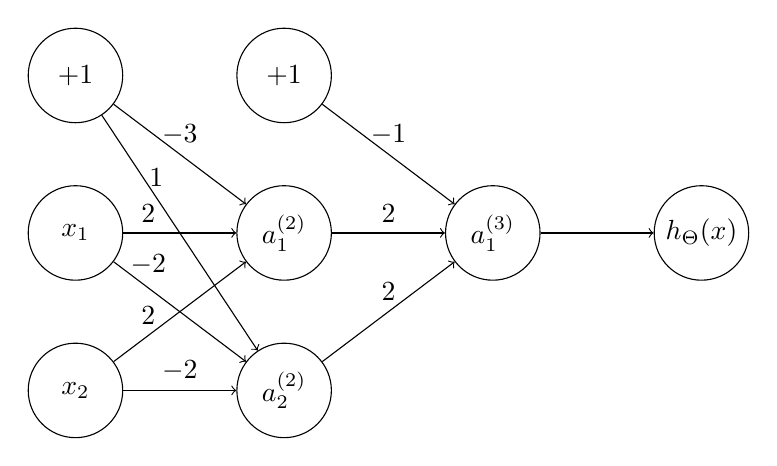
\begin{tikzpicture}[
    neuron/.style={circle,draw,inner sep=0pt,minimum size=12mm}
    ]
    
    \node (a12) at (0, 0) [neuron] {$a_1^{(2)}$};
    \node (a02) at (0, 2) [neuron] {$+1$};
    \node (a22) at (0, -2) [neuron] {$a_2^{(2)}$};
    \node (x0) at (-2.65, 2) [neuron] {$+1$};
    \node (x1) at (-2.65, 0) [neuron] {$x_1$};
    \node (x2) at (-2.65, -2) [neuron] {$x_2$};
    \node (a13) at (2.65, 0) [neuron] {$a_1^{(3)}$};
    \node (output) at (5.3, 0) [neuron] {$h_\Theta(x)$};
    \draw [->] (x0) to node [yshift=2.5mm] {$-3$} (a12);
    \draw [->] (x0) to node [xshift=-3mm, yshift=7mm] {$1$} (a22);
    \draw [->] (x1) to node [xshift=-4mm, yshift=2.5mm] {$2$} (a12);
    \draw [->] (x1) to node [xshift=-4mm, yshift=6mm] {$-2$} (a22);
    \draw [->] (x2) to node [xshift=-4mm, yshift=-0.5mm] {$2$} (a12);
    \draw [->] (x2) to node [yshift=2.5mm] {$-2$} (a22);
    \draw [->] (a02) to node [yshift=2.5mm] {$-1$} (a13);
    \draw [->] (a12) to node [yshift=2.5mm] {$2$} (a13);
    \draw [->] (a22) to node [yshift=2.5mm] {$2$} (a13);
    \draw [->] (a13) to (output);
  \end{tikzpicture}
   \end{center} 

  通过简单的计算我们得到,$a_1^{(2)}$ 计算得到的结果是 $AB$,
  $a_2^{(2)}$ 计算得到的结果是 $\overline{AB}$,$a_1^{(3)}$ 计算得到的结果是 $\overline{AB} + AB$,是我们需要的结果。
\end{example}

\subsection{神经网络解决多分类问题}
在神经网络中,我们可以通过将输出层的神经元个数设置为类别的个数,从而解决多分类问题。
例如,我们有三个类别,那么我们可以将输出层的神经元个数设置为 $3$,
并且将每个神经元的激活函数设置为 Sigmoid 函数,从而得到每个类别的概率。

之后,我们对所有输出层的输出值求 $\max$,得到最大的概率对应的类别即为预测结果。

\subsection{神经网络的代价函数}
在神经网络中,我们使用交叉熵作为代价函数:
假设 $h_\Theta(x) \in \mathbb{R}^K$,
$\left(h_\Theta(x)\right)_i$ 表示神经网络中输出向量的第 $i$ 个输出,即向量中的第 $i$ 项,则代价函数表示为
\begin{equation}
    \begin{aligned}
        J(\Theta) = &-\dfrac 1m\left[\sum\limits_{i=1}^m{\sum\limits_{k=1}^K{y_k^{(i)}\log (h_\Theta(x^{(i)})_k) + (1 - y_k^{(i)}) \log (1 - (h_\Theta(x^{(i)}))_k)}}\right] \\ 
        &+ \dfrac \lambda{2m}\sum\limits_{l=1}^{L-1}{\sum\limits_{i=1}^{s_l}{\sum\limits_{j=1}^{s_{l+1}}\left(\Theta_{ji}^{(l)}\right)^2}}
    \end{aligned}
\end{equation}

\begin{proof}
对于此函数,直观的理解是将其与逻辑回归的代价函数做对比,由于神经网络中输出是一个 $\mathbb{R}^K$ 的向量,
于是必须存在一个求和将这些输出单元的代价加起来,这就有了内层的求和号;

对于第 $k$ 个输出单元,它预测的类别是 $h_\Theta(x^{(i)})_k$,实际的类别是 $(y^{(i)})_k$,
将其在逻辑回归的代价函数中做替换即可得到神经网络代价函数中的前一项;

而后一项明显为 L2 正则项,逻辑回归中是将除 $\theta_0$ 以外的所有参数平方后求和,
类比到神经网络中,以 $a_1^{(i+1)}$ 举例,它会和 $a_1^{(i)}, a_2^{i}, \dots, a_{s_{i}}^{(i)}$ 这 $s_{i}$ 个神经元相连,
相连时的参数分别为 $\Theta_{11}^{(i)}, \Theta_{12}^{(i)}, \dots, \Theta_{1s_i}^{(i)}$,那么这个神经元表示的逻辑回归即为
\begin{equation}
    a_1^{(i+1)} = \sum\limits_{j=0}^{s_i}{\Theta_{1j}^{(i)}a_j^{(i)}}
\end{equation}
那么这一个逻辑回归对应的 L2 正则项为
\begin{equation}
    \sum\limits_{j=1}^{s_i}\left({\Theta_{1j}^{(i)}}\right)^2
\end{equation}
将第 $i+1$ 层的 $s_{i+1}$ 个神经元都考虑进来得到
\begin{equation}
    \sum\limits_{j=1}^{s_i}{\sum\limits_{k=1}^{s_{i+1}}\left({\Theta_{kj}^{(i)}}\right)^2}
\end{equation}
再把第 $1$ 层到第 $L-1$ 层考虑进来便得到神经网络代价函数中的后一项。
\end{proof}

\subsection{反向传播算法}
反向传播算法是一个让代价函数最小化的算法。
为了使用梯度下降法来找到 $\underset{\Theta}{\arg \min}\ J(\Theta)$,
我们需要计算 $J(\Theta)$ 和 $\dfrac{\partial}{\partial \Theta_{ij}^{(l)}}J(\Theta)$ 的值,从而能够使用梯度下降。

\subsubsection{每层只有一个神经元的情况}

考虑最后一层的激活值是如何计算的:
\begin{equation}
    a^{(L)} = g\left(\omega^{(L)}a^{(L-1)} + b^{(L)}\right) = g\left(z^{(L)}\right)
\end{equation}

这个过程如下图所示:
\begin{center}
    \begin{tikzpicture}[
        neuron/.style={circle,draw,inner sep=0pt,minimum size=12mm}
        ]
    
        \node (aL-1) at (0, 0) [neuron] {$a^{(L-1)}$};
        \node (wL) at (-2.65, 0) [neuron] {$\omega^{(L)}$};
        \node (bL) at (2.65, 0) [neuron] {$b^{(L)}$};
        \node (zL) at (0, -2.65) [neuron] {$z^{(L)}$};
        \node (aL) at (0, -5.3) [neuron] {$a^{(L)}$};
        \node (y) at (-2.65, -5.3) [neuron] {$y$};
        \node (C0) at (0, -7.95) [neuron] {$C_0$};
        \draw (wL) to (zL);
        \draw (aL-1) to (zL);
        \draw (bL) to (zL);
        \draw (zL) to (aL);
        \draw (y) to (C0);
        \draw (aL) to (C0);
      \end{tikzpicture}
\end{center}

下面假设代价函数为均方误差。考虑计算当 $\omega^{(L)}$ 变化时,代价函数的变化程度,即
\begin{equation}
    \dfrac{\partial}{\partial \omega^{(L)}} C_0
\end{equation}
根据求导的链式法则有
\begin{equation}
    \dfrac{\partial}{\partial \omega^{(L)}} C_0 = \dfrac{\partial z^{(L)}}{\partial \omega^{(L)}} 
    \cdot \dfrac{\partial a^{(L)}}{\partial z^{(L)}} \cdot \dfrac{\partial C_0}{\partial a^{(L)}}
\end{equation}
下面计算右侧各式的值:
\begin{equation}
    \begin{aligned}
        \dfrac{\partial C_0}{\partial a^{(L)}} &= \dfrac{\partial }{\partial a^{(L)}} \dfrac 12 \left(a^{(L)} - y\right)^2= \left(a^{(L)} - y\right) \\
        \\
        \dfrac{\partial a^{(L)}}{\partial z^{(L)}} &= \dfrac{\partial}{\partial z^{(L)}} g\left(z^{(L)}\right)= \dfrac{\partial}{\partial z^{(L)}} z^{(L)} \cdot g'\left(z^{(L)}\right) = g'\left(z^{(L)}\right) \\
        \\
        \dfrac{\partial z^{(L)}}{\partial \omega^{(L)}} &= \dfrac{\partial}{\partial \omega^{(L)}} \left(\omega^{(L)}a^{(L-1)} + b^{(L)}\right) = a^{(L-1)}
        \end{aligned}
\end{equation}

\subsubsection{每层有多个神经元的情况}
我们令 $j$ 表示最后一层的第 $j$ 个神经元,$k$ 表示倒数第二层的第 $k$ 个神经元,此时最后一层的代价为
\begin{equation}
    C_0 = \dfrac 12 \sum\limits_{j=0}^{s_L-1}{\left(a_j^{(L)} - y_j\right)^2}
\end{equation}
再次提醒,$\omega^{(L)}_{jk}$ 表示 $L - 1$ 层的第 $k$ 个神经元连向 $L$ 层的第 $j$ 个神经元的权重,与单神经元类似地,令
\begin{equation}
    z_j^{(L)} = \sum\limits_{k=0}^{s_{L-1}-1} {\omega_{jk}^{(L)}a_k^{(L-1)}} + b_j^{(L)}
\end{equation}
则最后一层的激活值为
\begin{equation}
    a_j^{(L)} = g\left(z_j^{(L)}\right)
\end{equation}
其中 $g(x)$ 为 Sigmoid 函数。再次利用求导的链式法则,我们得到
\begin{equation}
    \begin{aligned}
        \dfrac{\partial C_0}{\partial \omega^{(L)}} &= \sum\limits_{k=0}^{s_{L-1}-1}a_k^{(L-1)}g'\left(z^{(L)}\right)\left(a^{(L)} - y\right) \\
        \\
        \dfrac{\partial C_0}{\partial b^{(L)}} &= 1g'\left(z^{(L)}\right)\left(a^{(L)} - y\right) \\
        \\
        \dfrac{\partial C_0}{\partial a_k^{(L-1)}} &= \sum\limits_{j=0}^{s_L-1}\omega_{jk}^{(L)}g'\left(z^{(L)}\right)\left(a^{(L)} - y\right)
        \end{aligned}
\end{equation}

\subsubsection{梯度下降的具体过程}
\begin{itemize}
    \item 先进行一次前向传播
    \begin{equation}
        \begin{cases}
            z^{(l)} = \omega^{(l)}a^{(l-1)} + b^{(l)} \\
            a^{(l)} = g\left(z^{(l)}\right)
            \end{cases}
    \end{equation}
    \item 计算输出层误差方程,按定义有
    \begin{equation}
        \delta_j^{(L)} = \dfrac{\partial C}{\partial z_j^{(L)}}
    \end{equation}
    由求导的链式法则得到
    \begin{equation}
        \delta_j^{(L)} = \dfrac{\partial C}{\partial a_j^{(L)}} g'\left(z_j^{(L)}\right) \quad {(\text{BP}1)}
        \label{BP1} 
    \end{equation}
    写作矩阵形式为
    \begin{equation}
        \delta^{(L)} = \nabla_aC \odot g'\left(z^{(L)}\right)
    \end{equation}
    其中 $\odot$ 表示按元素的乘积,有时也被称为 Hadamard 乘积或 Schur 乘积。举例:
    \begin{equation*}
        \begin{bmatrix}1 \\ 2\end{bmatrix} \odot 
        \begin{bmatrix}3 \\ 4\end{bmatrix} = 
        \begin{bmatrix}1 * 3 \\ 2 * 4\end{bmatrix} = \begin{bmatrix}3 \\ 8\end{bmatrix}
    \end{equation*}
    \item 再通过下一层的误差 $\delta^{(l+1)}$ 表示当前层的误差 $\delta^{(l)}$
    \begin{equation}
        \delta^{(l)} = \left((\omega^{(l+1)})^\mathrm{T}\delta^{(l+1)}\right) \odot g'\left(z^{(l)}\right) \quad (\text{BP}2)
        \label{BP2}
    \end{equation}
    \item 通过梯度下降更新权重 $\omega$ 和偏置值 $b$
    \begin{equation}
        \begin{cases}
            \omega_{jk}^{(l)} := \omega_{jk}^{(l)} - a_k^{(l-1)}\delta_j^{(l)} \\
            \\
            b_j^{(l)} := b_j^{(l)} - \delta_j^{(l)}
        \end{cases}
    \end{equation}
\end{itemize}

\begin{proof}
   下面给出式 \ref{BP2} 的证明:
\begin{equation}
    \begin{aligned}
        \delta^{(l)} &= \dfrac{\partial C}{\partial z^{(l)}} \\
        \\
        &= \dfrac{\partial C}{\partial z^{(l+1)}} \cdot \dfrac{\partial z^{(l+1)}}{\partial a^{(l)}} \cdot \dfrac{\partial a^{(l)}}{\partial z^{(l)}} \\
        \\
        &= (\delta^{(l+1)} \cdot \omega^{(l+1)}) \odot g'\left(z^{(l)}\right)
    \end{aligned}
\end{equation}
由于 $\omega^{(l+1)}$ 维数为 $s_l \times s_{l+1}$,故上式也可以写作
\begin{equation}
    \delta^{(l)} = ((\omega^{l+1})^\mathrm{T}\delta^{(l+1)}) \odot g'\left(z^{(l)}\right)
\end{equation}
得证。 
\end{proof}

\subsection{梯度检查}

梯度检查是一个用来保证每次的前向传播、反向传播都是正确的算法。
当 $\theta \in \mathbb{R}^n$ 时,
此时 $\theta = \left[\theta_1, \theta_2, \dots, \theta_n\right]$,我们只需要对向量中每一个参数的偏导数都进行估计即可。具体地,
\begin{equation}
    \dfrac{\partial}{\partial \theta_i}J(\theta) = \lim\limits_{\epsilon \to 0} \dfrac{J(\dots, \theta_{i - 1}, \theta_i + \epsilon, \theta_{i+1}, \dots)
     - J(\dots, \theta_{i - 1}, \theta_i - \epsilon, \theta_{i+1}, \dots)}{2\epsilon}
\end{equation}

其中 $\epsilon$ 一般取 $10^{-4}$ 即可。

\textbf{在正式训练中不要使用梯度检查,因为计算代价相比于反向传播而言非常大。}

\subsection{随机初始化}
在神经网络中,对参数进行初始化时,我们需要使用随机初始化的思想。

具体地,令每个 $\Theta_{ij}^{(l)}$ 等于 $[-\epsilon, \epsilon]$ 内的一个随机数,即
\begin{equation}
    -\epsilon \leq \Theta_{ij}^{(l)} \leq \epsilon
\end{equation}

\subsection{总结}
\begin{itemize}
    \item 选择一个合适的神经网络架构:
    \begin{itemize}
        \item 输入层单元个数为特征向量的维度;
        \item 输出层单元个数为所要区分的类别个数。注意,每个数据的类别应当是一个\textbf{向量},而不是一个实数。
        \item 一般来说,默认只用一个隐藏层,如果使用多个隐藏层的话,默认每个隐藏层都具有相同数量的神经元。
    \end{itemize}
    \item 训练神经网络:
    \begin{itemize}
        \item 随机地初始化权重矩阵;
        \item 对于每个训练数据 $x^{(i)}$,执行前向传播以得到输出 $h_\Theta(x^{(i)})$;
        \item 计算代价函数 $J(\Theta)$;
        \item 执行反向传播计算所有的偏导数 $\dfrac{\partial}{\partial \Theta_{jk}^{(l)}}J(\Theta)$;
        \item 使用一次梯度检查来保证计算结果的正确性,然后禁用梯度检查;
        \item 通过梯度下降或其他方法求出 $\underset{\Theta}{\arg\min}\ J(\Theta)$。
    \end{itemize}
\end{itemize}

\section{卷积神经网络}
卷积神经网络(CNN)是一个专门用于图像处理的神经网络。

\subsection{卷积层}

在 CNN 中,我们设计一个特定大小的区域称作“感受野”(Receptive field),
每一个神经元都只需要关心自己的感受野里面有什么东西。举例:
感受野为 $3\times3$,则一个神经元只需要输入一个 $3\times3\times3=27$ 维的向量,权重数目明显减少;

多个感受野的范围是可以重叠的,不同的神经元也可以有相同的感受野。

最经典的感受野设定:

\begin{itemize}
    \item 考虑一张图片所有的通道,而不是只考虑部分通道;
    \item 感受野的长和宽被称作 kernel size,如上方讨论的感受野的 kernel size 为 $3\times3$,一般不会设置很大的 kernel size;
    \item 同一个感受野会对应一组神经元,例如 64 个或 128 个;
    \item 对于两个相邻的感受野,将偏移量(采样间隔)称为 stride(步幅),这是一个超参数,通常不会很大,一般设置为 1 或 2 即可;
    \item 当感受野超出图像范围时,我们可以向感受野中做 padding(填补),一般补充为 0。
\end{itemize}

相同的特征可能会出现在图像的不同区域中,
但是这些相同的特征对应的是不同的神经元,但他们做的是相同的工作。我们是否需要让每一个区域都放若干个对应不同特征的神经元?

考虑共享参数,两个对应不同感受野的对应相同特征的神经元,让他们共享相同的参数,这样参数的数量将会大大减少。
由于两个神经元对应的感受野不同,他们的输入不一致,所以它们的输出也不会一样。

常见的共享参数的方法:对于同一层上的神经元,每一个感受野对应的神经元都只有一组参数,这组参数被称作 filter。

加入上述两个限制之后,我们得到的就是卷积层 Convolutional Layer。

另一种常见的解释方式是,定义若干个 $3 \times 3 \times \text{channel}$ 的 filter,将每个 filter 在输入的图片上做卷积操作,每次将 filter 移动 stride 长度,
如果超出图像范围时,我们可以选择进行 padding。

\begin{figure}[htbp]
    \centering
    \caption{卷积示意图}
    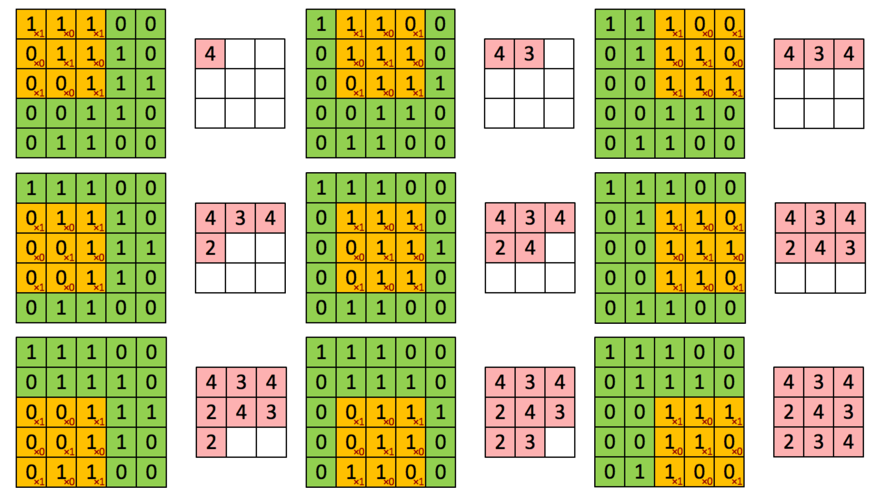
\includegraphics[scale = 0.5]{convolution.png}
\end{figure}

卷积后得到的结果被称做 Feature map。卷积之后得到的 Feature map 可以看做是一张新的图片,
只是通道数不再是输入的通道数(1 个通道 + n 个卷积核得到 n 个通道)。

当然,卷积层也是可以叠加很多层的。卷积层叠的越多,考虑的范围就会越来越大。

有时还可以在卷积之后做一次 ReLU 操作,使 Feature map 中不出现负数值结果:
\begin{equation}
    \operatorname{ReLU}(x) = \max(0, x)
\end{equation}

卷积后图像大小由下面的公式进行计算:
\begin{equation}
    \operatorname{new\_feature\_size} = \left\lfloor\operatorname{img\_size} - 
    \operatorname{filter\_size}\right\rfloor / \operatorname{stride} + 1
\end{equation}

其中,img\_size 表示原图大小,filter\_size 表示卷积核大小,stride 表示卷积核移动的步长。

\begin{example}
    输入图片规格经过预处理后尺寸为 $227 \times 227 \times 3$,
    卷积核大小为 $11 \times 11 \times 3$,步长为 $4$,则经过卷积后得到的特征图大小为
    \begin{equation*}
        \left\lfloor227 - 11\right\rfloor / 4 + 1 = 55
    \end{equation*}
    即得到的特征图的尺寸为 $55 \times 55 \times 3$。
\end{example}

\subsection{池化层}
我们观察到,有时对于一张图片,我们对其做下采样(按照一定规律在图片中采样,使图片尺寸缩小),得到的图片特征是不变的。

根据此,我们可以对卷积得到的 Feature map 通过池化层进行压缩。

我们选取一个窗口大小(通常是 $2\times2$ 或 $3\times3$),然后选择步幅(通常选择 2),
对每个窗口中的所有数取 $\max$,最终得到一个特征不变但是尺寸变小的一个 Feature map。

池化可以减少运算量,但相应的可能会损失掉一些细微的特征。池化可以改善结果,使之不容易过拟合。

经过几次卷积和池化后,我们将得到的 Feature map “拉直”(flatten)为一个向量,丢进全连接层,最后通过一个 softmax 回归器来得到最终的投票结果。

\begin{figure}[htbp]
    \centering
    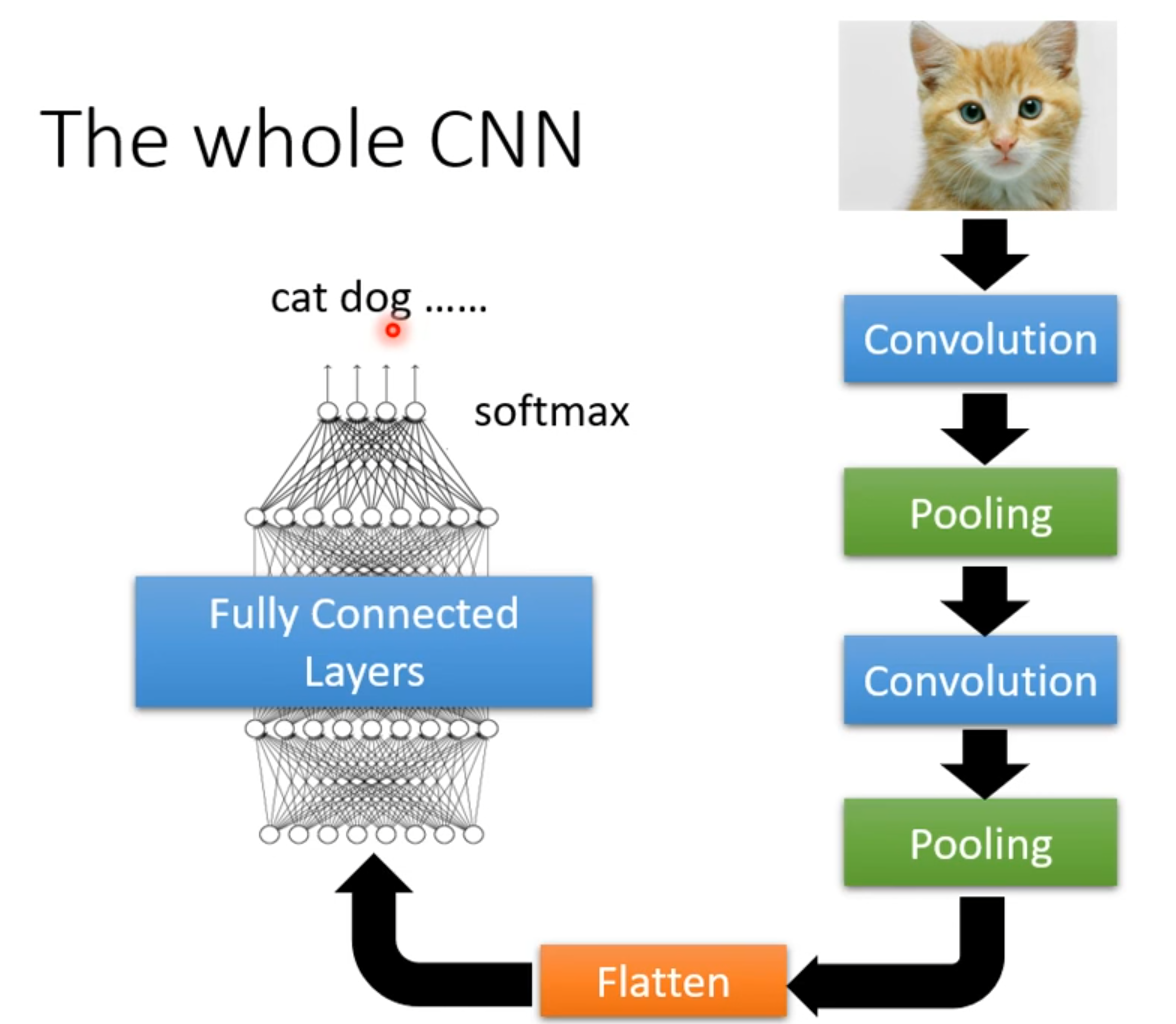
\includegraphics[scale = 0.25]{CNN.png}
\end{figure}

\subsection{超参数}
\begin{itemize}
    \item 卷积层:卷积核的数量;卷积核的大小;卷积核移动的步长
    \item 池化层:窗口的大小;窗口移动的步长
    \item 全连接层:神经元个数
\end{itemize}

\subsection{卷积神经网络的推广}
不仅是图片,卷积神经网络也可以用于其他类型的数据,比如文本、语音、视频等。
只要数据可以用矩阵表示,就可以用卷积神经网络来处理。

\section{稀疏自编码器}
\subsection{自编码器}
传统反向神经网络缺点:
\begin{itemize}
    \item 梯度越来越稀疏(梯度弥散):从顶层越往下,误差校正信号越来越小;
    \item 容易收敛到局部最小值,尤其是从远离最优区域开始的时候(将参数初始化为随机值会导致这种情况发生);
    \item 只能进行有监督训练,但大部分的数据是没有标签的,而人类的大脑可以从没有标签的数据中学习。
\end{itemize}

\textbf{1986} 年,\textbf{Rumelhart} 提出了自动编码器的概念,并将其用于高维复杂数据的处理,促进了神经网络的发展。
自编码神经网络是一种\textbf{无监督}(自监督)学习算法,它使用了反向传播算法,
并让\textbf{目标值等于输入值},即自编码神经网络尝试学习一个 $h_{W, b}(x) \approx x$ 的函数。

自编码器分类:
\begin{itemize}
    \item 浅层自编码(Autoencoder)
    \item 稀疏自编码(Sparse Autoencoder)
    \item 栈式自编码(Stacked Autoencoder)
    \item 去噪自编码(Denoising Autoencoder)
    \item 变分自编码(Variational Autoencoder)
\end{itemize}

自编码器的共同点:学习一个\textbf{与输入相同的输出},并尽可能的让其具有较强的\textbf{泛化能力}。

自编码器的构成:
\begin{itemize}
    \item 编码器是把高维度数据\textbf{有损的}映射成低维度数据,
    减少数据量,要实现这种映射关系需要学习数据间的相关性,对输入 $x$ 编码,得到新的特征 $y$;
    \item 解码器和编码器完全相反,是把低维度数据映射成高维度数据,\textbf{增加数据量},
    使经过压缩的数据恢复成原来的样子,即利用新的特征 $y$,得到一个重构的数据 $x'$;
    \item 损失函数用来衡量由于压缩而损失掉的信息。编码器和解码器一般都是参数化的方程,
    且关于损失函数\textbf{可导},典型的情况是使用最小均方误差
    \begin{equation}
        \text{MSE} = \dfrac 1n \sum\limits_{i=1}^n (x - x')^2
    \end{equation}
\end{itemize}

\subsection{深度自编码器}
\textbf{2006} 年,\textbf{Hinton} 对原型自动编码器的结构进行了改进,
进而产生了 DAE,先用\textbf{无监督逐层贪心训练算法}完成对隐含层的\textbf{预训练},
然后用\textbf{反向传播}算法对整个神经网络进行系统性参数优化调整,
显著降低了神经网络的训练复杂程度,有效改善了反向传播算法容易陷入局部最小的不良状况。

将三层浅层自编码器扩展成具有多个隐藏层的编码器即为深度自编码器,能更好的学习数据更高维度的特征。

\subsubsection{逐层学习}
在深度自编码器中,对其中的多个隐藏层,我们需要进行逐层自编码学习。
具体地,每一个编码层中都会包含一个解码器,用来输出当前层的解码结果,我们贪心地希望每一层的解码结果都与前一层向其输入的结果尽可能的相似:
\begin{figure}[htbp]
    \centering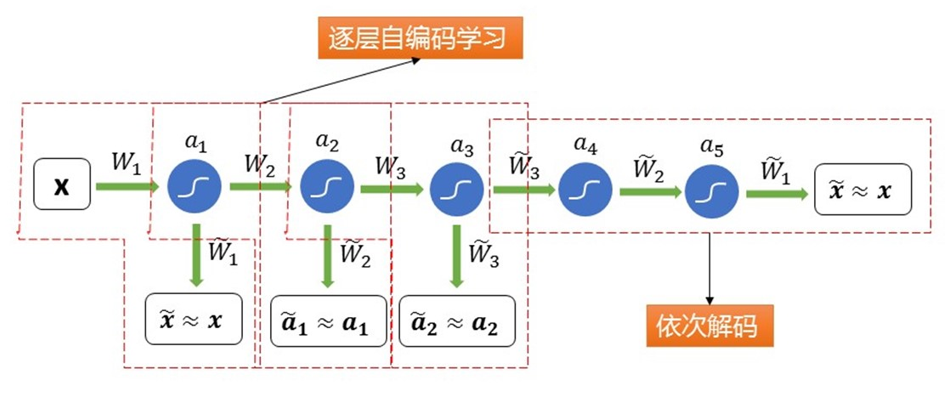
\includegraphics[scale = 0.4]{DAE.png}
\end{figure}

深度自编码器特点:具有强大的\textbf{表达能力}及深度神经网络的\textbf{所有优点}。
它通常能够获取到输入的“层次性分组”或者“部分-整体分解”结构。自编码器倾向于学习得到能更好地\textbf{表示输入数据的特征}。

\subsection{稀疏表示}
我们可以寻找一个系数矩阵 $u$ 和一个字典矩阵 $V$,使得 $V \times u$ 尽可能的还原 $x$,
且 $u$ 尽可能地稀疏,则 $u$ 就是 $x$ 的稀疏表示。我们将一个大矩阵变成两个小矩阵,从而达到压缩的目的。
\begin{figure}[htbp]
    \centering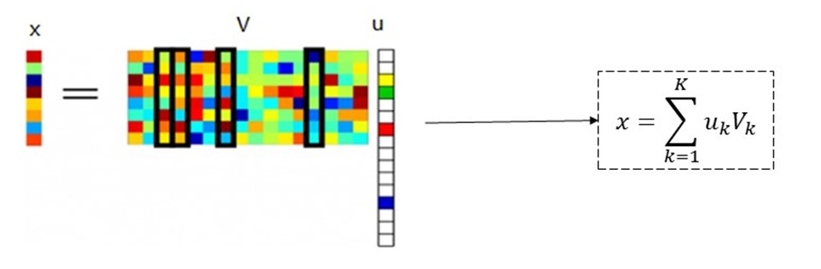
\includegraphics[scale = 0.5]{sparse.png}
\end{figure}

给定数据集 $\left\{\boldsymbol{x}_1, \boldsymbol{x}_2, \dots, \boldsymbol{x}_m\right\}$,字典学习的最简单形式为
\begin{equation}
    J(\mathbf B, \boldsymbol{\alpha}) = \min_{\mathbf B, \boldsymbol{\alpha}_i} \sum_{i=1}^m
    \left\|x_i - \mathbf B \boldsymbol{\alpha}_i\right\|_2^2 
    + \lambda\sum_{i=1}^m\left\|\boldsymbol{\alpha}_i\right\|_1  
\end{equation}

其中 $\mathbf B \in \mathbb{R}^{d \times k}$ 为字典矩阵,$k$ 称为字典的\textbf{词汇量},通常由用户指定。
$\boldsymbol{\alpha}_i \in \mathbb{R}^k$ 则是样本 $\boldsymbol{x}_i \in \mathbb{R}^d$ 的稀疏表示。
显然,上式的第一项是希望 $\boldsymbol{\alpha}_i$ 能较好地重构 $\boldsymbol{x}_i$,
第二项则是希望 $\boldsymbol{\alpha}_i$ 尽量稀疏,可以再加入一项 $+ \beta\sum_r\sum_c \mathbf B_{rc}^2$,表示希望字典中每项也尽可能小。

为了较为简单的最小化上述二元函数,我们通过变量交替优化的策略来进行:
\begin{itemize}
    \item 首先随机初始化字典矩阵 $\mathbf B$;
    \item 然后通过梯度下降,得到 $\mathbf B$ 确定时使得函数 $J(\cdot, \cdot)$ 取得最小值时的 $\boldsymbol{\alpha}$;
    \item 再通过梯度下降,得到 $\boldsymbol{\alpha}$ 确定时使得函数 $J(\cdot, \cdot)$ 取得最小值时的 $\mathbf B$;
    \item 不断重复上述两步,直至结果确定。
\end{itemize}

\subsection{稀疏自编码}

一个神经网络中,使得神经元在大部分的时间内都是被\textbf{抑制}的限制称为\textbf{稀疏性限制}。

考虑一个最简单的自编码器,其神经网络只有三层,那么 $a_j^{(2)}$ 表示隐藏层中的隐藏神经元 $j$ 的激活值,
但这种表示方法无法表示是哪一个输入 $x$ 带来的激活值,所以我们改用 $a_j^{(2)}(x)$ 表示在给定输入为 $x$ 的情况下,
隐藏层中的隐藏神经元 $j$ 的激活值。

令
\begin{equation}
    \hat{\rho}_j = \dfrac 1m \sum_{i=1}^m{a_j^{(2)}(x^{(i)})}
\end{equation}

表示隐藏神经元 $j$ 在 $m$ 个输入样本上的平均激活度。

再近似的加入一条限制:$\hat{\rho}_j = \rho$,其中 $\rho$ 被称为稀疏性参数。
为了满足这一限制,将会在优化目标函数中加入一个惩罚因子,
这将惩罚那些 $\hat{\rho}_j$ 和 $\rho$ 有显著不同的情况,从而使得隐藏神经元的平均活跃度保持在较小范围内。

\subsubsection{KL 散度}
定义两分布 $P$,$Q$ 之间的相对熵(KL 散度)为
\begin{equation}
    D(P\|Q) = \sum_xE\left[\ln p(x) - \ln q(x)\right] = \sum_xp(x) \ln \dfrac{p(x)}{q(x)}
\end{equation}

其中 $p(x)$,$q(x)$ 为两分布的概率密度函数。
相对熵可以解释为“通过 $q$ 的编码去编码 $p$后,信息丢失数的期望”,可以用相对熵来表示两个分布之间的差异。

把隐层的每个神经元的激活和未激活态看做服从\textbf{二项分布},
则 KL 散度可以表示为一个以 $\rho$ 为均值和一个以 $\hat{\rho}_j$ 为均值的两个二项分布之间的相对熵:
\begin{equation}
    \operatorname{KL}(\rho \| \hat{\rho}_j) = 
    \rho\ln\dfrac{\rho}{\hat{\rho}_j} + (1 - \rho) \ln \dfrac{1 - \rho}{1 - \hat{\rho}_j}
\end{equation}

KL 散度的三个特点:
\begin{itemize}
    \item $\operatorname{KL}(\rho \| \hat{\rho}_j) \geq 0$,当且仅当 $\rho = \hat{\rho}_j$ 时取等号;
    \item 非对称性:$\operatorname{KL}(\rho\|\hat{\rho}_j) \neq \operatorname{KL}(\hat{\rho}_j\|\rho)$;
    \item 当 $\hat\rho_j \to 0 \text{ or } 1$ 时,$\operatorname{KL}(\rho \| \hat\rho_j) \to +\infty$。
\end{itemize}

现在,代价函数可以表示为
\begin{equation}
    J_{\text{sparse}}(\mathbf B, \boldsymbol{\alpha}) 
    = J(\mathbf B, \boldsymbol{\alpha}) + \beta\sum_{j=1}^{s_2}\operatorname{KL}(\rho\|\hat{\rho}_j)
\end{equation}

注意到
\begin{equation}
    \dfrac{\partial \operatorname{KL}(\rho \| \hat{\rho}_j)}{\partial \hat{\rho}_j} 
    = -\dfrac{\rho}{\hat{\rho}_j} + \dfrac{1 - \rho}{1 - \hat{\rho}_j}
\end{equation}

于是在神经网络的反向传播中,当前层误差 $\delta^{(l)}$ 更新为
\begin{equation}
    \delta^{(l)} = \left((\omega^{(l+1)})^\mathrm{T}\delta^{(l+1)} 
    + \beta\left(-\dfrac{\rho}{\hat{\rho}_j} + \dfrac{1 - \rho}{1 - \hat{\rho}_j}\right)\right) 
    \odot g'\left(z^{(l)}\right)
\end{equation}

即可,其中 $l = n_l - 1, n_l - 2, \dots, 2$。
注意,在进行稀疏自编码器的训练过程中,必须要先进行一次前向传播以得到所有神经元的平均激活度 $\hat{\rho}$。
\end{document}